% !TeX root = ../../Book4.tex
% 纲要标题：## 第10章　矩映射与辛约化
% 纲要位置：几何学计划纲要.md，第 3846 行。
% 正文状态：初稿；尚未正式审核。

% 纲要内容开始
% 
% > 本章目标与证明范围：完整证明正则值上自由固有作用的约化定理；先处理矩映射的存在与等变性障碍，再讨论商空间，避免把每个辛作用都当作 Hamilton 作用。
% 
% 纲要内容结束

\chapter{矩映射与辛约化}
\label{g4:ch:10}
\BookChapterNumber{g4:ch:10}

\begin{chapterabstract}
对称性使 Hamilton 系统具有守恒量，也使同一个运动状态可以有许多等价描述。矩映射把群的各个无穷小方向组织成函数族；分量方程的可解性与等变性分别受到一形式周期和 Lie 代数余循环的限制。本章据此研究矩映射水平集，证明自由固有作用下的闭二形式下降与非退化性，完整建立正则辛约化定理。余切丛、复射影空间、余伴随轨道及分阶段约化给出可计算的模型。最后通过有限稳定子与零水平锥面，区分轨形商、辛层和约化光滑结构，并给出一般奇异约化定理的明确引用版本。
\end{chapterabstract}

\begin{learninggoals}
\begin{itemize}
	\item 核对左作用基本场、Hamilton 场与 Poisson 括号的符号，计算线动量、角动量与圆作用的矩映射。
	\item 分别判断矩映射分量的存在与等变性，计算常数调整及两重存在障碍。
	\item 由矩映射微分确定水平集切空间和辛正交，证明基本闭二形式下降到光滑商。
	\item 完整证明正则值上的辛约化定理，并解释一般值为何须除以该值的余伴随稳定子。
	\item 计算余切丛、射影空间和余伴随轨道的约化辛形式，核验分阶段约化的相容条件。
	\item 计算有限群局部商与奇异锥的辛层，辨别底层拓扑和约化光滑结构，并掌握一般奇异约化定理的适用范围。
\end{itemize}
\end{learninggoals}

取 \(\mathbb C^{n+1}\) 中固定长度的向量。如果只关心它所确定的复直线，那么相差一个共同相位的向量应视为同一个状态。长度条件先把空间限制到球面，相位等价再把球面变成复射影空间。这两个操作各少一个实维数，最后留下偶数维空间。原来的标准辛形式能否同时通过这两步，成为射影空间上的辛形式？

\ProseParagraphBreak

一般情形中，固定长度被固定矩映射的值代替，共同相位被群轨道代替。矩映射方程保证，水平集上原形式的退化方向恰好是需要被除去的轨道方向。商的光滑性则需要另一个条件：群作用自由且固有。只有把微分形式的退化与商空间的几何分别说明，再证明它们相容，约化才能产生新的辛流形。

\ProseParagraphBreak

构造之前还要解决矩映射本身是否存在的问题。前章的环面平移已经表明，辛向量场可以没有全局 Hamilton 函数；辛平面的二维平移又表明，各方向都有生成函数时，这些函数仍可能不能组成等变矩映射。相应的周期与余循环计算说明了约化定理为何以 Hamilton 作用为前提。

\ProseParagraphBreak

本章使用第七章的辛正交与线性约化、第九章的 Hamilton 场及 Poisson 括号，以及第一卷第17章已证的自由固有作用商定理。余伴随作用及轨道辛形式在本章恢复所需定义与计算，主干不以先读第九章的退化 Poisson 部分为条件。矩映射和正则约化的参考为 Cannas da Silva 的第5.6、6.1–6.2节；\secref{g4:sec:1004}的一般分层结论按该节列出的版本引用 Sjamaar 与 Lerman 的论文。\cite[第153--157、160--165页]{Cannas2006Symplectic}

% !TeX root = ../../Book4.tex
% 纲要标题：### 10.1 群作用和矩映射
% 纲要位置：几何学计划纲要.md，第 3850 行。
% 正文状态：初稿；尚未正式审核。

% 纲要内容开始
% 
% * 基本向量场及作用侧别
% * Hamilton 作用与矩映射分量
% * 等变性和加常数的自由
% * Lie 代数余循环与存在障碍
% 
% 纲要内容结束

\section{群作用和矩映射}
\label{g4:sec:1001}

平移与旋转都能同时作用于许多轨迹。若每个群方向都由一个 Hamilton 函数产生，把这些函数按方向排列，就得到取值于 Lie 代数对偶的映射。困难在于两次选择：闭一形式未必有全局原函数，而已有的原函数也未必能同时按群的乘法规律变换。本节把这两件事分别检验。流形均取有限维、无边界、Hausdorff、第二可数；在讨论常数与障碍时另明确连通性。

\subsection{基本向量场及作用侧别}
\label{g4:subsec:1001:01}

设 Lie 群 \(G\) 光滑左作用于 \(M\)，记 \(a_g(x)=g\cdot x\)，于是 \(a_{gh}=a_g\circ a_h\)。其 Lie 代数记为 \(\mathfrak g\)。对 \(\xi\in\mathfrak g\)，沿正向单参数子群运动，定义\term[jibenxiangliangchang]{基本向量场}[fundamental vector field]
\begin{equation}\label{g4:eq:1001:fundamental-field}
	\xi_M(x)=\left.\frac{\mathrm{d}}{\mathrm{d}t}\right|_{t=0}\exp(t\xi)\cdot x.
\end{equation}
这里的流对一切实时间都有定义，就是 \(a_{\exp(t\xi)}\)。基本场来自一个已经给定的群作用，因而自动完备。

\begin{proposition}\label{g4:prop:1001:fundamental-fields}
	设有限维实 Lie 群 \(G\) 光滑左作用于光滑流形 \(M\)，并采用式\eqref{g4:eq:1001:fundamental-field}。则 \(\xi\mapsto\xi_M\) 线性，且
	\begin{equation}\label{g4:eq:1001:fundamental-bracket}
		(a_g)_*\xi_M=(\operatorname{Ad}_g\xi)_M,
		\qquad [\xi_M,\eta_M]=-[\xi,\eta]_M.
	\end{equation}
\end{proposition}
\begin{proof}
	第一卷命题17.1.2给出这些公式。这里恢复决定符号的两步。轨道映射 \(g\mapsto g\cdot x\) 在单位元的微分就是 \(\xi\mapsto\xi_M(x)\)，故它线性。恒等式
	\[
		g\exp(t\xi)\cdot x=\exp(t\operatorname{Ad}_g\xi)\cdot(g\cdot x)
	\]
	给出推前公式。沿 \(\xi_M\) 的流拉回 \(\eta_M\)，得到 \((\operatorname{Ad}_{\exp(-t\xi)}\eta)_M\)。第一卷命题16.1.7说明 \(\operatorname{ad}_\xi\eta=[\xi,\eta]\)，所以对 \(t\) 在零点求导便得负号。
\end{proof}

例如 \(\operatorname{GL}(m,\mathbb R)\) 左作用于 \(\mathbb R^m\) 时，矩阵 \(A\) 的基本场为 \(x\mapsto Ax\)。按向量场括号的坐标公式，\([Ax,Bx]=(BA-AB)x\)，确实是 \(-[A,B]x\)。若从一个右作用改写成左作用，应使用 \(g\cdot x=x\cdot g^{-1}\)，相应基本场也改变符号。

\begin{definition}\label{g4:def:1001:symplectic-action}
	设 \((M,\omega)\) 为辛流形。若光滑左作用 \(a:G\times M\to M\) 满足 \(a_g^*\omega=\omega\) 对每个 \(g\in G\) 成立，则称它为\term[xinqunzuoyong]{辛作用}[symplectic action]。
\end{definition}

辛作用的每个基本场都是辛向量场，因此 \(\iota_{\xi_M}\omega\) 是闭一形式。反过来，若全部基本场都保辛，只能先推出单位连通分支 \(G^0\) 保辛：每个指数元保辛，第一卷命题16.2.5再说明有限个指数元生成 \(G^0\)。其他连通分支中的元素仍须逐一满足作用保持辛形式的要求。

\subsection{Hamilton 作用与矩映射分量}
\label{g4:subsec:1001:02}

对固定方向 \(\xi\)，求生成函数就是解 \(\mathrm{d}H_\xi=\iota_{\xi_M}\omega\)。由于右边对 \(\xi\) 线性，希望左边也由一份线性的函数族给出。选一组基并对基方向选择原函数，就能把逐个方向的解组织起来。

\begin{definition}\label{g4:def:1001:moment-map}
	设 \(G\) 辛作用于 \((M,\omega)\)。若光滑映射 \(\mu:M\to\mathfrak g^*\) 的每个分量 \(\mu^\xi(x)=\langle\mu(x),\xi\rangle\) 满足
	\begin{equation}\label{g4:eq:1001:moment-equation}
		\mathrm{d}\mu^\xi=\iota_{\xi_M}\omega
		\qquad(\xi\in\mathfrak g),
	\end{equation}
	则称 \(\mu\) 为该作用的\term[juyingshe]{矩映射}[moment map]。本节先把分量方程与下文的等变条件分开；有些文献将等变性一并纳入矩映射的定义。
\end{definition}

\begin{proposition}\label{g4:prop:1001:component-existence}
	设 \(G\) 辛作用于非空连通辛流形 \((M,\omega)\)。满足分量方程的矩映射存在，当且仅当每个 \(\iota_{\xi_M}\omega\) 恰当；只检查 \(\mathfrak g\) 的一组基就足够。任意两个这样的映射之差是 \(\mathfrak g^*\) 中的一个常向量。
\end{proposition}
\begin{proof}
	必要性直接来自分量方程。反之，取基 \(e_1,\ldots,e_k\) 与对偶基 \(e^1,\ldots,e^k\)，选择 \(\mathrm{d}H_j=\iota_{(e_j)_M}\omega\)，定义 \(\mu=\sum_jH_je^j\)。它光滑；对 \(\xi=\sum_j\xi^je_j\)，分量为 \(\mu^\xi=\sum_j\xi^jH_j\)，满足所需方程。若 \(\nu\) 也是解，则每个 \(\nu^{e_j}-\mu^{e_j}\) 的微分为零，在连通 \(M\) 上为常数。这些常数合成一个固定的 \(b\in\mathfrak g^*\)。
\end{proof}

\begin{example}\label{g4:exm:1001:linear-angular}
	在 \(\mathrm{T}^*\mathbb R^n\) 上，\(\omega=\sum_j\mathrm{d}q^j\wedge\mathrm{d}p_j\)。平移 \(a\cdot(q,p)=(q+a,p)\) 的基本场为 \(\sum_ja^j\partial_{q^j}\)，故 \(\mu(q,p)=p\)。在三维情形，旋转 \(R\cdot(q,p)=(Rq,Rp)\) 的基本场为 \((a\times q,a\times p)\)，其中将 \(\mathfrak{so}(3)\) 识别为带叉积括号的 \(\mathbb R^3\)。直接求微分得
	\[
		\mathrm{d}\bigl(a\cdot(q\times p)\bigr)
		=(a\times q)\cdot\mathrm{d}p-(a\times p)\cdot\mathrm{d}q.
	\]
	所以矩映射为 \(\mu(q,p)=q\times p\)。前者收集线动量，后者收集角动量；矩映射把这些随方向线性变化的量写成一个对象。
\end{example}

\begin{example}\label{g4:exm:1001:circle-sign}
	在 \(\mathbb C\) 上写 \(z=x+\mathrm{i}y\)、\(\omega=\mathrm{d}x\wedge\mathrm{d}y\)，圆周参数取 \(\mathbb R/(2\pi\mathbb Z)\)。正旋转 \(e^{\mathrm{i}t}z\) 的基本场为 \(-y\partial_x+x\partial_y\)，收缩得到 \(-\mathrm{d}(|z|^2/2)\)，故矩映射是 \(-|z|^2/2\)。负旋转 \(e^{-\mathrm{i}t}z\) 的矩映射则是 \(|z|^2/2\)。后面用球面构造射影空间时采用后一种作用。
\end{example}

矩映射分量还说明对称性为什么产生守恒量。若 \(H\) 在群作用下不变，则沿任一基本场的导数为零，于是
\[
	X_H\mu^\xi=\{\mu^\xi,H\}=-\xi_MH=0.
\]
因而 \(\mu\) 沿 \(H\) 的每条轨迹保持常值。反过来，若全部分量沿 \(H\) 的轨迹不变，则 \(\xi_MH=0\) 对每个 \(\xi\) 成立，故 \(H\) 被 \(G^0\) 保持；当 \(G\) 连通时，它被整个群保持。这个对应称为 Hamilton 形式的\term[noetherdingli]{Noether 定理}[Noether's theorem]。\footnote{Emmy Amalie Noether（1882--1935），德国数学家，研究抽象代数，并建立连续对称性与守恒律之间的关系。}上述计算就是此处所需版本的完整证明；流只在实际存在的时间区间内使用。\cite[第5.6节，定理5.18，第155--156页]{Cannas2006Symplectic}

\subsection{等变性和加常数的自由}
\label{g4:subsec:1001:03}

群作用不仅移动点，也改变所观察的 Lie 代数方向。由第一卷的伴随表示，在对偶上取
\begin{equation}\label{g4:eq:1001:coadjoint}
	\langle\operatorname{Ad}_g^*\lambda,\xi\rangle
	=\langle\lambda,\operatorname{Ad}_{g^{-1}}\xi\rangle.
\end{equation}
这就是余伴随作用\termidx[yubansuizuoyong]{余伴随作用}；公式中的逆元保证 \(\operatorname{Ad}_{gh}^*=\operatorname{Ad}_g^*\operatorname{Ad}_h^*\)。它也恢复了\secref{g4:sec:0904}所用的约定。

\begin{definition}\label{g4:def:1001:equivariant}
	设 \(G\) 辛作用于 \((M,\omega)\)。若矩映射 \(\mu\) 还满足
	\begin{equation}\label{g4:eq:1001:equivariance}
		\mu(g\cdot x)=\operatorname{Ad}_g^*\mu(x)
		\qquad(g\in G,\ x\in M),
	\end{equation}
	则称它为\term[dengbianjuyingshe]{等变矩映射}[equivariant moment map]。存在等变矩映射的作用称为\term[Hamiltonzuoyong]{Hamilton 作用}[Hamiltonian action]，相应数据 \((M,\omega,G,\mu)\) 称为 Hamilton \(G\) 空间。
\end{definition}

线动量与角动量都满足等变性：平移群交换，所以其余伴随作用平凡，而 \(p\) 在平移下不变；旋转保持叉积，所以 \((Rq)\times(Rp)=R(q\times p)\)。交换群的等变条件总是矩映射的不变性。\cite[定义5.16及其例，第154--155页]{Cannas2006Symplectic}

\begin{proposition}\label{g4:prop:1001:equivariance-bracket}
	设 \(G\) 辛作用于辛流形 \((M,\omega)\)，\(\mu\) 满足分量方程。若 \(\mu\) 等变，则
	\begin{equation}\label{g4:eq:1001:infinitesimal-equivariance}
		\{\mu^\xi,\mu^\eta\}=\mu^{[\xi,\eta]}
		\qquad(\xi,\eta\in\mathfrak g).
	\end{equation}
	若 \(G\) 连通，则反过来也成立。
\end{proposition}
\begin{proof}
	在等变式中取 \(g=\exp(t\eta)\)，与 \(\xi\) 配对后在零点求导。左边是 \(\eta_M\mu^\xi=\{\mu^\xi,\mu^\eta\}\)，右边由 \(\operatorname{Ad}_{\exp(-t\eta)}\xi\) 的导数得到 \(\mu^{[\xi,\eta]}\)，证明必要性。

	反之，固定 \(\eta\) 与 \(x\)，令 \(u(t)=\mu(\exp(t\eta)\cdot x)\)。括号等式给出
	\[
		\frac{\mathrm{d}}{\mathrm{d}t}\langle u(t),\xi\rangle
		=\langle u(t),[\xi,\eta]\rangle.
	\]
	这是 \(\mathfrak g^*\) 上的常系数线性方程；\(\operatorname{Ad}_{\exp(t\eta)}^*\mu(x)\) 满足相同方程及初值，故二者相等。第一卷命题16.2.5保证连通 \(G\) 中每个元素都是有限个指数元的乘积，逐次使用此等式便得到整个群的等变性。
\end{proof}

\begin{proposition}\label{g4:prop:1001:constant-freedom}
	设 \(G\) Hamilton 作用于非空连通辛流形 \((M,\omega)\)，\(\mu\) 为等变矩映射。则全部等变矩映射恰为
	\[
		\mu+b,\qquad b\in(\mathfrak g^*)^G
		=\{b:\operatorname{Ad}_g^*b=b\text{ 对每个 }g\in G\}.
	\]
	若 \(G\) 连通，则 \((\mathfrak g^*)^G\) 是消灭 \([\mathfrak g,\mathfrak g]\) 的协向量空间。
\end{proposition}
\begin{proof}
	分量方程的全部解已经由\cref{g4:prop:1001:component-existence}确定为 \(\mu+b\)。将其代入等变式，恰好剩下 \(b=\operatorname{Ad}_g^*b\)。在单位元求导，得到 \(b([\xi,\eta])=0\)。反之，此条件使 \(b\) 沿每个余伴随指数曲线不变，连通性与指数生成性给出整个群的不变性。
\end{proof}

因此交换群可任意平移矩映射的常数，而连通且 \([\mathfrak g,\mathfrak g]=\mathfrak g\) 的群至多有一个等变矩映射。常数平移会改变哪一张水平集被称为零水平集；在约化问题中，必须把所选矩映射和约化值一起说明。

\begin{proposition}\label{g4:prop:1001:normalization}
	设 \(G\) 辛作用于非空连通辛流形 \((M,\omega)\)，且分量方程有解。以下任一归一化都给出等变矩映射：若 \(G\) 有共同不动点 \(x_0\)，要求 \(\mu(x_0)=0\)；若 \(M\) 闭，要求 \(\int_M\mu\,\omega^n=0\)，其中 \(2n=\dim M\)，积分逐分量定义。
\end{proposition}
\begin{proof}
	对任意 \(g\)，推前公式及保辛性给出
	\[
		\mathrm{d}(\mu^\xi\circ a_g)
		=\iota_{(\operatorname{Ad}_{g^{-1}}\xi)_M}\omega
		=\mathrm{d}\mu^{\operatorname{Ad}_{g^{-1}}\xi}.
	\]
	故 \(\mu\circ a_g-\operatorname{Ad}_g^*\mu\) 在连通 \(M\) 上为常向量。在不动点处，两项都为零；在闭流形情形，两项的积分都为零，因为 \(a_g\) 保持辛体积。于是此常向量为零。归一化可分别通过减去 \(\mu(x_0)\) 或 \(\int_M\mu\omega^n/\int_M\omega^n\) 达到。
\end{proof}

\subsection{Lie 代数余循环与存在障碍}
\label{g4:subsec:1001:04}

先把求原函数的障碍写成一个线性映射：
\begin{equation}\label{g4:eq:1001:first-obstruction}
	\mathcal O:\mathfrak g\longrightarrow H^1_{\mathrm{dR}}(M),
	\qquad \xi\longmapsto[\iota_{\xi_M}\omega].
\end{equation}
\cref{g4:prop:0903:infinitesimal-obstruction}及基本场的括号公式表明，\(\mathcal O([\xi,\eta])=0\)。所以它只依赖于交换化空间 \(\mathfrak g/[\mathfrak g,\mathfrak g]\)。\(\mathcal O=0\) 恰好保证分量方程有解；例如 \(H^1_{\mathrm{dR}}(M)=0\) 或 \(\mathfrak g=[\mathfrak g,\mathfrak g]\) 时，这一障碍自动消失。

\begin{example}\label{g4:exm:1001:torus-obstruction}
	在 \(\mathbb T^2=\mathbb R^2/\mathbb Z^2\) 上取 \(\omega=\mathrm{d}q\wedge\mathrm{d}p\)。圆周群 \(\mathbb R/\mathbb Z\) 沿 \(q\) 方向平移，基本场为 \(\partial_q\)，对应闭一形式 \(\mathrm{d}p\)。它在 \(p\) 方向的圆周上积分为 \(1\)，故不恰当。这个辛作用没有满足分量方程的矩映射，正是前章通量障碍的无穷小表现。
\end{example}

即使 \(\mathcal O=0\)，已选函数的 Poisson 括号还可能差一个常数。设 \(M\) 连通，选择分量方程的解 \(\mu\)，定义
\begin{equation}\label{g4:eq:1001:cocycle}
	c(\xi,\eta)=\{\mu^\xi,\mu^\eta\}-\mu^{[\xi,\eta]}.
\end{equation}

\begin{proposition}\label{g4:prop:1001:lie-cocycle}
	设 \(G\) 辛作用于非空连通辛流形 \((M,\omega)\)，\(\mu\) 满足分量方程。式\eqref{g4:eq:1001:cocycle}为与点无关的交替双线性实函数，并满足
	\begin{equation}\label{g4:eq:1001:cocycle-identity}
		c([\xi,\eta],\zeta)+c([\eta,\zeta],\xi)+c([\zeta,\xi],\eta)=0.
	\end{equation}
	将 \(\mu\) 改成 \(\mu+b\) 后，\(c\) 改成 \(c-b([\ ,\ ])\)。若 \(G\) 连通，则存在等变矩映射，当且仅当 \(\mathcal O=0\)，且由任一分量解所得的 \(c\) 可以写成 \(b([\xi,\eta])\)。
\end{proposition}
\begin{proof}
	由\cref{g4:prop:0902:hamiltonian-bracket}，
	\[
		X_{\{\mu^\xi,\mu^\eta\}}
		=-[\xi_M,\eta_M]=[\xi,\eta]_M
		=X_{\mu^{[\xi,\eta]}}.
	\]
	因此 \(\mathrm{d}c(\xi,\eta)=0\)，连通性使其为常数。双线性与交替性直接来自两个括号。

	在函数括号的 Jacobi 恒等式中代入 \(\mu^\xi,\mu^\eta,\mu^\zeta\)。每个内层括号等于 \(\mu^{[\xi,\eta]}+c(\xi,\eta)\)；常数与函数的括号为零，外层括号再用同一分解。含 \(\mu\) 的三项由 \(\mathfrak g\) 的 Jacobi 恒等式相消，余下正是式\eqref{g4:eq:1001:cocycle-identity}。

	加常数不改变 Poisson 括号，却使 \(\mu^{[\xi,\eta]}\) 增加 \(b([\xi,\eta])\)，所以得到变换公式。最后，\(\mathcal O=0\) 给出初始分量解；能选 \(b\) 消去 \(c\) 恰好使其保持 Lie 括号，再用\cref{g4:prop:1001:equivariance-bracket}得到等变性。反向取等变矩映射时，两个障碍都为零。
\end{proof}

满足式\eqref{g4:eq:1001:cocycle-identity}的交替双线性函数称为取平凡实系数的\term[liedaishuerciyuxunhuan]{Lie 代数二次余循环}[Lie algebra 2-cocycle]。它们构成的空间记为 \(Z^2(\mathfrak g;\mathbb R)\)；形如 \(b([\xi,\eta])\) 的余循环构成子空间 \(B^2(\mathfrak g;\mathbb R)\)。Jacobi 恒等式直接保证这确是子空间包含。商空间
\[
	H^2(\mathfrak g;\mathbb R)=Z^2(\mathfrak g;\mathbb R)/B^2(\mathfrak g;\mathbb R)
\]
称为二次\term[liedaishushangtongdiao]{Lie 代数上同调}[Lie algebra cohomology]；只把 \(c\) 改为另一代表，不改变障碍类 \([c]\)。通常上链微分写作 \((\delta b)(\xi,\eta)=-b([\xi,\eta])\)，它给出的余边界子空间相同。这里的上同调属于 Lie 代数，与第一重障碍所在的流形 de Rham 上同调是不同对象。\cite[第5.6节，第156--157页]{Cannas2006Symplectic}

\begin{example}\label{g4:exm:1001:translation-cocycle}
	令交换群 \(\mathbb R^2\) 平移辛平面 \((\mathbb R^2_{q,p},\mathrm{d}q\wedge\mathrm{d}p)\)。对基方向 \(e_1,e_2\)，可取 \(\mu^{e_1}=p\)、\(\mu^{e_2}=-q\)。每个基本场都是 Hamilton 场，但
	\[
		c(e_1,e_2)=\{p,-q\}=1.
	\]
	Lie 代数交换，所以 \(b([e_1,e_2])=0\) 对每个 \(b\) 成立；任何常数调整都不能消去 \(c\)。因此此作用没有等变矩映射。这与单方向平移有矩映射并不冲突：同时组织两个方向时，新增了它们的括号相容条件。
\end{example}

\begin{example}\label{g4:exm:1001:so3-existence}
	设连通群 \(\operatorname{SO}(3)\) 辛作用于连通辛流形。\(\mathfrak{so}(3)\cong\mathbb R^3\) 的括号为叉积，故 \([\mathfrak g,\mathfrak g]=\mathfrak g\)，第一重障碍为零。任意交替双线性函数 \(c\) 都可唯一写成 \(b(\xi\times\eta)\)：只需按 \(e_1\times e_2=e_3\) 及其循环式指定 \(b\) 在基上的值。这直接消去第二重障碍。所以每个这样的辛作用都是 Hamilton 作用，且等变矩映射唯一。这个三维计算不需要调用一般半单 Lie 代数的上同调定理。
\end{example}

还可以直接看到不连通群带来的额外条件。对分量解 \(\mu\)，令
\[
	\sigma(g)=\mu(g\cdot x)-\operatorname{Ad}_g^*\mu(x).
\]
归一化命题中的微分计算说明它与 \(x\) 无关，且光滑。逐次作用给出
\begin{equation}\label{g4:eq:1001:group-cocycle}
	\sigma(gh)=\sigma(g)+\operatorname{Ad}_g^*\sigma(h),\qquad
	\sigma_{\mu+b}(g)=\sigma(g)+b-\operatorname{Ad}_g^*b.
\end{equation}
这样的变换律称为群的\term[qunyiciyuxunhuan]{一次余循环}[group 1-cocycle]。等变性恰好是 \(\sigma=0\)，而
\[
	\left.\frac{\mathrm{d}}{\mathrm{d}t}\right|_{0}
	\langle\sigma(\exp(t\eta)),\xi\rangle=c(\xi,\eta).
\]
所以 \(c=0\) 只控制单位分支。具体地，\(G=\mathbb R\times\mathbb Z\) 在辛平面上作用为 \((s,k)\cdot(q,p)=(q+s,p+k)\)。它的 Lie 代数只有 \(q\) 平移方向，分量解 \(\mu=p\) 的二次余循环为零；但 \(\sigma(s,k)=k\)，而交换群下加常数不能改变 \(\sigma\)。这个例子说明，完整的 Hamilton 作用还须满足离散分支的等变条件。
% 纲要条目排为编号小节标题，并进入目录与书签；说明段仍保留于纲要注释中。

% !TeX root = ../../Book4.tex
% 纲要标题：### 10.2 约化的线性和微分几何
% 纲要位置：几何学计划纲要.md，第 3857 行。
% 正文状态：初稿；尚未正式审核。

% 纲要内容开始
% 
% * 水平集的切空间
% * 辛正交与轨道方向
% * 闭二形式下降
% * 非退化性和商光滑性
% * Marsden–Weinstein 约化的完整证明
% 
% 纲要内容结束

\section{约化的线性和微分几何}
\label{g4:sec:1002}

固定矩映射的一个值，相当于给运动状态施加若干守恒量约束；再把对称群能够互相移动的状态视为相同，就得到约化空间。辛形式不能直接下降到任意轨道商：沿轨道改变切向量代表时，配对的值可能随之改变。本节将说明，矩映射水平集恰好使需要商掉的方向成为限制二形式的核。线性代数解决配对是否良定义，自由固有作用保证商是光滑流形，局部截面则把逐点配对组织成光滑闭形式。

\subsection{水平集的切空间}
\label{g4:subsec:1002:01}

沿用\cref{g4:def:1001:moment-map}的约定。有限维实 Lie 群 \(G\) 左作用于辛流形 \((M,\omega)\)，其 Lie 代数为 \(\mathfrak g\)，正向指数产生基本场 \(\xi_M\)。对矩映射 \(\mu:M\to\mathfrak g^*\)，记 \(\mu^\xi=\langle\mu,\xi\rangle\)，则
\[
	\mathrm{d}\mu^\xi=\iota_{\xi_M}\omega,
	\qquad
	\langle\mathrm{d}\mu_x(v),\xi\rangle=\omega_x(\xi_M(x),v).
\]
右侧同时记录了约束微分和轨道方向；这是约化证明中的基本等式。

\begin{proposition}\label{g4:prop:1002:moment-differential}
	设有限维实 Lie 群 \(G\) 辛作用于无边界辛流形 \((M,\omega)\)，且 \(\mu:M\to\mathfrak g^*\) 满足矩映射方程。令
	\[
		\rho_x:\mathfrak g\longrightarrow\mathrm{T}_xM,
		\quad \rho_x(\xi)=\xi_M(x),
		\qquad V_x=\operatorname{im}\rho_x,
		\quad\mathfrak g_x=\ker\rho_x.
	\]
	这里 \(V_x\) 是轨道切空间，\(\mathfrak g_x\) 是无穷小稳定子。则
	\begin{equation}\label{g4:eq:1002:moment-kernel-image}
		\ker\mathrm{d}\mu_x=V_x^\omega,
		\qquad
		\operatorname{im}\mathrm{d}\mu_x=\mathfrak g_x^\circ,
	\end{equation}
	其中 \(\mathfrak g_x^\circ\subset\mathfrak g^*\) 为消灭 \(\mathfrak g_x\) 的泛函空间。因此 \(x\) 是 \(\mu\) 的正则点，当且仅当 \(\mathfrak g_x=0\)。若 \(a\) 是正则值且 \(Z_a=\mu^{-1}(a)\ne\varnothing\)，则 \(Z_a\) 是余维 \(\dim G\) 的嵌入子流形，并且
	\begin{equation}\label{g4:eq:1002:level-tangent}
		\mathrm{T}_xZ_a=\ker\mathrm{d}\mu_x=V_x^\omega.
	\end{equation}
\end{proposition}
\begin{proof}
	对 \(v\in\mathrm{T}_xM\)，\(\mathrm{d}\mu_x(v)=0\) 等价于它与每个 \(\xi\in\mathfrak g\) 的配对为零，也就是 \(\omega_x(\xi_M(x),v)=0\) 对所有 \(\xi\) 成立。这给出第一个等式。

	把 \(\mathrm{d}\mu_x\) 转置，所得映射把 \(\xi\) 送到一形式 \(\omega_x(\rho_x\xi,\cdot)\)。辛形式的非退化性说明其核恰为 \(\mathfrak g_x\)，故 \(\mathrm{d}\mu_x\) 的秩等于 \(\dim\mathfrak g-\dim\mathfrak g_x\)。另一方面，若 \(\xi\in\mathfrak g_x\)，上面的配对恒为零，所以 \(\operatorname{im}\mathrm{d}\mu_x\subseteq\mathfrak g_x^\circ\)。两边维数相等，得到第二个等式和正则点判据。

	第一卷定理11.4.4的正则水平集定理给出最后的结论。具体说，在每个原像点附近，淹没标准形把 \(\mu-a\) 写成前 \(\dim G\) 个坐标的投影；令这些坐标为零就得到水平集，其切空间正是该投影的核。
\end{proof}

自由性蕴含 \(\mathfrak g_x=0\)。确实，若 \(\xi_M(x)=0\)，基本场积分曲线的唯一性说明 \(\exp(t\xi)x=x\) 对所有 \(t\) 成立；自由性迫使 \(\exp(t\xi)=e\)，在零时刻求导便得 \(\xi=0\)。反方向只能排除无穷小稳定子，不能排除离散的非平凡稳定子。

\begin{example}\label{g4:exm:1002:regular-not-free}
	在 \(\mathbb C\setminus\{0\}\) 上取 \(\omega=\mathrm{d}x\wedge\mathrm{d}y\)，令圆周按 \(e^{it}\cdot z=e^{ikt}z\) 作用，其中整数 \(k\ge2\)。基本场为 \(k(-y\partial_x+x\partial_y)\)，矩映射可取
	\[
		\mu(z)=-\frac{k}{2}|z|^2.
	\]
	其微分在这个空间处处非零，所以每个非空水平都是正则水平；但每一点的稳定子都有 \(k\) 个元素，作用并不自由。这个例子区分了水平集的光滑性与商映射所需的自由性。
\end{example}

\subsection{辛正交与轨道方向}
\label{g4:subsec:1002:02}

现在假设矩映射等变，即 \(\mu(gx)=\operatorname{Ad}_g^*\mu(x)\)，其中余伴随作用按前节的含 \(g^{-1}\) 约定定义。零在这个线性作用下固定，所以 \(Z=\mu^{-1}(0)\) 被整个 \(G\) 保持。于是每个基本场在 \(Z\) 上切向，轨道方向 \(V_x\) 包含于 \(\mathrm{T}_xZ\)。

\begin{proposition}\label{g4:prop:1002:zero-level-kernel}
	设有限维实 Lie 群 \(G\) 辛作用于无边界辛流形 \((M,\omega)\)，\(\mu:M\to\mathfrak g^*\) 是等变矩映射，\(0\) 是正则值且 \(Z=\mu^{-1}(0)\ne\varnothing\)。令 \(i:Z\hookrightarrow M\)，\(\beta=i^*\omega\)。则对每个 \(x\in Z\)，
	\begin{equation}\label{g4:eq:1002:zero-level-kernel}
		V_x\subseteq V_x^\omega=\mathrm{T}_xZ,
		\qquad
		(\mathrm{T}_xZ)^\omega=V_x,
		\qquad
		\ker\beta_x=V_x.
	\end{equation}
	特别地，轨道切空间各向同性，水平集切空间余各向同性。
\end{proposition}
\begin{proof}
	等变性给出 \(V_x\subseteq\mathrm{T}_xZ\)，而\cref{g4:prop:1002:moment-differential}给出 \(\mathrm{T}_xZ=V_x^\omega\)。\cref{g4:prop:0701:orthogonal-dimensions}的双重辛正交等式说明 \((\mathrm{T}_xZ)^\omega=(V_x^\omega)^\omega=V_x\)。限制型的核是
	\[
		\mathrm{T}_xZ\cap(\mathrm{T}_xZ)^\omega
		=\mathrm{T}_xZ\cap V_x=V_x,
	\]
	得到全部结论。
\end{proof}

也可直接检查轨道上的配对。由\cref{g4:prop:1001:equivariance-bracket}，
\[
	\omega_x(\xi_M(x),\eta_M(x))
	=\{\mu^\xi,\mu^\eta\}(x)
	=\langle\mu(x),[\xi,\eta]\rangle.
\]
它在零水平上为零。这个计算说明等变性怎样使群方向成为允许商掉的各向同性方向；而核的完整描述还需要上面的双重正交论证。

\ProseParagraphBreak

因此，每个 \(x\in Z\) 都给出一个辛向量空间
\[
	\mathrm{T}_xZ/V_x=V_x^\omega/V_x,
	\qquad
	\overline\omega_x([u],[v])=\omega_x(u,v).
\]
这是\cref{g4:thm:0701:linear-reduction}的逐点应用。下一步要确认：不同点得到的商空间能够成为同一个光滑商流形的切空间，而且这些配对随商点光滑变化。

\subsection{闭二形式下降}
\label{g4:subsec:1002:03}

先把形式下降的问题与辛非退化性分开。设 \(G\) 在流形 \(P\) 上自由且固有地作用，商映射记为 \(\pi:P\to B=P/G\)。第一卷定理17.2.6说明 \(B\) 是光滑流形，\(\pi\) 是满射淹没；第一卷引理17.2.5的局部乘积给出每点附近的光滑截面。截面选择一个轨道代表，但形式的值必须与这个选择无关。

\begin{definition}\label{g4:def:1002:basic-form}
	对有限维实 Lie 群 \(G\) 在无边界光滑流形 \(P\) 上的光滑作用，若微分形式 \(\alpha\) 满足 \(\iota_{\xi_P}\alpha=0\) 对所有 \(\xi\in\mathfrak g\) 成立，则称它为\term[shuipingxingshi]{水平形式}[horizontal form]。若它还对整个群不变，即 \(L_g^*\alpha=\alpha\) 对所有 \(g\in G\) 成立，则称它为\term[jibenxingshi]{基本形式}[basic form]。
\end{definition}

这里“水平”表示只要一个输入沿轨道，形式就为零，并没有为轨道方向选择一个补空间。水平性消除切向量提升的歧义；不变性消除轨道代表的歧义。

\begin{proposition}\label{g4:prop:1002:basic-descent}
	设有限维实 Lie 群 \(G\) 自由且固有地光滑作用于无边界流形 \(P\)，两者均为 Hausdorff、第二可数。赋予 \(B=P/G\) 自由固有商的光滑结构，并记商映射为 \(\pi\)。对 \(k\ge1\) 及 \(\alpha\in\Omega^k(P)\)，存在 \(\overline\alpha\in\Omega^k(B)\) 满足
	\begin{equation}\label{g4:eq:1002:basic-descent}
		\pi^*\overline\alpha=\alpha
	\end{equation}
	当且仅当 \(\alpha\) 为基本形式；存在时 \(\overline\alpha\) 唯一。并且 \(\overline\alpha\) 闭当且仅当 \(\alpha\) 闭。
\end{proposition}
\begin{proof}
	若 \(\alpha=\pi^*\overline\alpha\)，则 \(\pi\circ L_g=\pi\) 给出不变性，而 \(\mathrm{d}\pi(\xi_P)=0\) 给出水平性。

	反过来，给定 \(b\in B\) 与 \(u_1,\ldots,u_k\in\mathrm{T}_bB\)，选择 \(x\in\pi^{-1}(b)\)，并借淹没性取 \(v_j\in\mathrm{T}_xP\)，使 \(\mathrm{d}\pi_x(v_j)=u_j\)。定义
	\[
		\overline\alpha_b(u_1,\ldots,u_k)
		=\alpha_x(v_1,\ldots,v_k).
	\]
	局部乘积中 \(\pi\) 是忘掉群因子的投影，因此 \(\ker\mathrm{d}\pi_x\) 正是基本场值张成的轨道切空间。改变任一提升只增加一个这样的向量，水平性使右侧不变。若改取另一代表 \(x'=gx\)，可用 \(\mathrm{d}L_g(v_j)\) 作提升；群不变性又使右侧不变。这证明定义良好，并给出拉回等式。

	取任一光滑局部截面 \(s:U\to P\)，则这个逐点定义在 \(U\) 上恰为 \(s^*\alpha\)，所以光滑。不同截面的拉回一致，已经由刚才的代表与提升无关性保证，因而这些局部形式粘成整体形式。任何满足拉回等式的形式都必须在 \(U\) 上等于 \(s^*\alpha\)，所以唯一。

	同样的局部截面说明 \(\pi^*\) 在所有次数上单射：若 \(\pi^*\gamma=0\)，则 \(\gamma|_U=s^*\pi^*\gamma=0\)。拉回与外微分交换，故
	\[
		\pi^*\mathrm{d}\overline\alpha
		=\mathrm{d}\pi^*\overline\alpha
		=\mathrm{d}\alpha.
	\]
	单射性给出两个闭性条件的等价。
\end{proof}

这条判据要求整个群的不变性。若 \(G\) 连通，闭形式的水平性通过 Cartan 公式给出 \(\mathcal L_{\xi_P}\alpha=0\)，沿基本场流积分并用第一卷命题16.2.5的指数生成性，可得到群不变性；若群不连通，仅有无穷小不变性不能控制其他连通分支。

\begin{example}\label{g4:exm:1002:descent-conditions}
	对 \(\mathbb R\) 在 \(\mathbb R_t\times\mathbb R_x\times\mathbb R_y\) 上沿 \(t\) 的平移，形式 \(\mathrm{d}t\wedge\mathrm{d}x\) 闭且不变，却不水平，因为插入 \(\partial_t\) 得到 \(\mathrm{d}x\)。所以它不下降到 \((x,y)\) 平面。

	再令离散群 \(\mathbb Z\) 在 \(\mathbb R^2\) 上按 \(m\cdot(x,y)=(x+m,y)\) 作用。这个作用自由且固有；由于群的 Lie 代数为零，每个形式都满足水平条件。但闭形式 \(e^x\mathrm{d}x\wedge\mathrm{d}y\) 在平移一次后乘以 \(e\)，因此不下降到圆柱 \((\mathbb R/\mathbb Z)\times\mathbb R\)。
\end{example}

\subsection{非退化性和商光滑性}
\label{g4:subsec:1002:04}

固有性的定义约束映射 \((g,x)\mapsto(gx,x)\)：若出发点和到达点都限制在紧集内，群参数也不能逃逸。自由固有商定理的证明正是先用逆函数定理找到横截面，再用这个条件排除远处群元素把横截面送回自身。局部乘积 \(G\times S\cong GS\) 随后提供商坐标和截面。不同轨道的分离性来自轨道等价关系闭；商投影是开映射，故源的可数基给出商的可数基。这些步骤保证商满足 Hausdorff 性与第二可数性，既有局部坐标也有正确的整体拓扑。

\ProseParagraphBreak

现在设 \(\beta\) 已经下降。商上的形式可能仍退化：水平性只说明轨道方向包含在 \(\ker\beta\) 中，只有当它们恰为全部核时，取商才能消除所有退化方向。

\begin{proposition}\label{g4:prop:1002:quotient-nondegeneracy}
	设有限维实 Lie 群 \(G\) 自由且固有地光滑作用于无边界流形 \(P\)，两者均为 Hausdorff、第二可数。设 \(\beta\) 为 \(P\) 上的基本闭二形式，\(\overline\beta\) 是它在 \(B=P/G\) 上的下降形式。则
	\begin{equation}\label{g4:eq:1002:quotient-tangent}
		\mathrm{T}_{[x]}B\cong
		\mathrm{T}_xP/\mathrm{T}_x(Gx),
		\qquad
		\ker\overline\beta_{[x]}
		\cong\ker\beta_x/\mathrm{T}_x(Gx).
	\end{equation}
	因此 \(\overline\beta\) 是辛形式，当且仅当 \(\ker\beta_x=\mathrm{T}_x(Gx)\) 对每个 \(x\in P\) 成立。
\end{proposition}
\begin{proof}
	第一卷定理17.2.6给出商流形与满射淹没 \(\pi\)。在局部乘积坐标中，\(\mathrm{d}\pi_x\) 忘掉群方向，所以其核是 \(\mathrm{T}_x(Gx)\)；线性同态定理给出第一项同构。

	若 \(u=\mathrm{d}\pi_x(v)\)，则 \(u\) 与全部商切向量的 \(\overline\beta\) 配对为零，当且仅当 \(\beta_x(v,w)=0\) 对全部 \(w\in\mathrm{T}_xP\) 成立，因为 \(\mathrm{d}\pi_x\) 满射。这等价于 \(v\in\ker\beta_x\)。水平性又保证 \(\mathrm{T}_x(Gx)\subseteq\ker\beta_x\)，从而得到第二项同构。闭性已由\cref{g4:prop:1002:basic-descent}证明，故核为零恰好是辛条件。
\end{proof}

这里没有假定群紧。若 \(G\) 紧，则作用自动固有：给定 \(P\times P\) 中紧集 \(C\)，其第二投影为紧集 \(K\)，\(C\) 在作用映射 \((g,x)\mapsto(gx,x)\) 下的原像是 \(G\times K\) 的闭子集，所以紧。非紧群则须实际检查固有性，不能从自由性推断。

\subsection{Marsden–Weinstein 约化的完整证明}
\label{g4:subsec:1002:05}

把水平集上的核计算与形式下降合在一起，就得到\term[MarsdenWeinsteinyuehuadingli]{Marsden--Weinstein 约化定理}[Marsden--Weinstein reduction theorem]。\footnote{Jerrold Eldon Marsden（1942--2010），加拿大出生、长期在美国工作的数学家，研究几何力学、辛约化与动力系统。}下面先处理零值；它对整个余伴随作用固定，所以全部群方向都留在同一个水平集内。

\begin{theorem}[Marsden--Weinstein 约化]\label{g4:thm:1002:symplectic-reduction}
	设 \(G\) 为 \(r\) 维实 Lie 群，\((M^{2n},\omega)\) 为无边界辛流形，二者均为 Hausdorff、第二可数。设 \(G\) 在 \(M\) 上光滑辛作用，且有等变矩映射 \(\mu:M\to\mathfrak g^*\)。假设 \(0\) 是正则值，\(Z=\mu^{-1}(0)\ne\varnothing\)，并且 \(G\) 在 \(Z\) 上的限制作用自由且固有。则
	\[
		M_{\mathrm{red}}=Z/G
	\]
	在商拓扑下是 \(2n-2r\) 维无边界光滑流形，商映射 \(\pi:Z\to M_{\mathrm{red}}\) 是满射淹没。存在唯一辛形式 \(\omega_{\mathrm{red}}\) 使
	\begin{equation}\label{g4:eq:1002:reduction-pullback}
		\pi^*\omega_{\mathrm{red}}=i^*\omega,
		\qquad i:Z\hookrightarrow M.
	\end{equation}
	逐点地，\(\mathrm{T}_{[x]}M_{\mathrm{red}}\) 与 \(V_x^\omega/V_x\) 辛同构。
\end{theorem}
\begin{proof}
	正则水平集定理使 \(Z\) 成为 \(2n-r\) 维嵌入子流形。等变性使 \(Z\) 对 \(G\) 不变，因此题设的限制作用有定义。自由固有商定理给出 \(Z/G\) 的光滑结构和满射淹没 \(\pi\)，维数再减去 \(r\)，得到 \(2n-2r\)。

	令 \(\beta=i^*\omega\)。因为作用保辛且 \(Z\) 不变，\(\beta\) 对整个 \(G\) 不变。对 \(x\in Z\)、\(v\in\mathrm{T}_xZ\)，矩映射方程给出
	\[
		\beta_x(\xi_M(x),v)
		=\omega_x(\xi_M(x),v)
		=\mathrm{d}\mu^\xi_x(v)=0,
	\]
	所以 \(\beta\) 水平；\(\mathrm{d}\beta=i^*\mathrm{d}\omega=0\)，所以它闭。\cref{g4:prop:1002:basic-descent}于是给出唯一光滑闭二形式 \(\omega_{\mathrm{red}}\)，满足所需拉回等式。

	由\cref{g4:prop:1002:zero-level-kernel}，\(\ker\beta_x=V_x\)，而自由作用下 \(V_x=\mathrm{T}_x(Gx)=\ker\mathrm{d}\pi_x\)。\cref{g4:prop:1002:quotient-nondegeneracy}遂给出 \(\omega_{\mathrm{red}}\) 非退化。最后，\(\mathrm{T}_xZ=V_x^\omega\) 和拉回等式说明商切空间上的配对恰为 \([u],[v]\mapsto\omega_x(u,v)\)，就是线性约化的辛同构。
\end{proof}

称 \((M_{\mathrm{red}},\omega_{\mathrm{red}})\) 为在零值处的\term[xinyuehuakongjian]{辛约化空间}[symplectic reduced space]，也称辛商。若作用在水平集上自由，\cref{g4:prop:1002:moment-differential}已经保证零是正则值；定理仍将正则性列出，以明确水平集与商流形两个构造分别使用的条件。紧群版本及线性证明可对照 Cannas da Silva 的定理6.1、引理6.3--6.4与命题6.5。这里用第一卷的自由固有商定理处理非紧群。\cite[第6.1节，第160--163页]{Cannas2006Symplectic}

% !TeX root = ../Book4.tex
\begin{figure}[htbp]
	\centering
	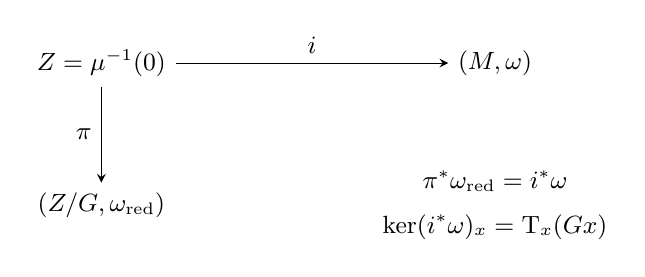
\begin{tikzpicture}[font=\small,>=stealth]
		\node (Z) at (0,1.5) {\(Z=\mu^{-1}(0)\)};
		\node (M) at (5,1.5) {\((M,\omega)\)};
		\node (B) at (0,-0.3) {\((Z/G,\omega_{\mathrm{red}})\)};
		\draw[->] (Z)--node[above] {\(i\)} (M);
		\draw[->] (Z)--node[left] {\(\pi\)} (B);
		\node[align=center] at (5,-0.3) {\(\pi^*\omega_{\mathrm{red}}=i^*\omega\)\\[5pt]\(\ker(i^*\omega)_x=\mathrm{T}_x(Gx)\)};
	\end{tikzpicture}
	\caption[水平集与轨道商]{先把辛形式限制到矩映射的零水平，再沿群轨道取商。限制型的核恰为商映射消去的方向，所以商上的形式非退化。}
	\label{g4:fig:1002:reduction-diagram}
\end{figure}


\begin{example}\label{g4:exm:1002:translation-reduction}
	在 \(\mathbb R^{2n}_{q,p}\) 中，让 \(G=\mathbb R^r\)、\(r\le n\)，平移前 \(r\) 个位置坐标。作用自由。按第一卷命题17.2.2的序列判据，它也固有：若 \(x_j\to x\)、\(t_jx_j\to y\)，群参数 \(t_j\) 等于两个点前 \(r\) 个位置坐标的差，因而收敛。矩映射为 \(\mu=(p_1,\ldots,p_r)\)，所以
	\[
		Z=\{p_1=\cdots=p_r=0\},\qquad
		Z/G\cong\mathbb R^{2(n-r)}.
	\]
	商映射保留 \((q^{r+1},\ldots,q^n,p_{r+1},\ldots,p_n)\)，约化形式为
	\[
		\omega_{\mathrm{red}}=\sum_{j=r+1}^n\mathrm{d}q^j\wedge\mathrm{d}p_j.
	\]
	水平约束先去掉 \(r\) 个动量方向，轨道商再去掉与之配对的 \(r\) 个位置方向。\(r=n\) 时约化空间为一点，其零二形式在零维切空间上非退化。
\end{example}

非零值的差别在于水平集未必被整个群保持。对 \(a\in\mathfrak g^*\)，定义余伴随稳定子
\[
	G_a=\{g\in G:\operatorname{Ad}_g^*a=a\}.
\]
它是闭子群，第一卷定理16.3.6赋予它嵌入 Lie 子群结构。其 Lie 代数为
\begin{equation}\label{g4:eq:1002:coadjoint-stabilizer-algebra}
	\mathfrak g_a=\{\xi\in\mathfrak g:
	\langle a,[\eta,\xi]\rangle=0\text{ 对所有 }\eta\in\mathfrak g\}.
\end{equation}
确实，\(\left.\frac{\mathrm{d}}{\mathrm{d}t}\right|_0\operatorname{Ad}_{\exp(t\xi)}^*a\) 与 \(\eta\) 的配对是 \(-\langle a,[\xi,\eta]\rangle\)。这个导数为零时，表示的单参数群规律使整个曲线的导数为零，因此 \(\exp(t\xi)\) 对所有 \(t\) 固定 \(a\)；反向由求导得到。闭子群定理中的指数判据便给出所列 Lie 代数。

\begin{theorem}\label{g4:thm:1002:nonzero-reduction}
	设 \(G\) 为有限维实 Lie 群，\((M^{2n},\omega)\) 为无边界辛流形，二者均为 Hausdorff、第二可数。设 \(G\) 辛作用于 \(M\)，\(\mu:M\to\mathfrak g^*\) 为等变矩映射。若 \(a\) 为正则值、\(Z_a=\mu^{-1}(a)\ne\varnothing\)，并且 \(G_a\) 在 \(Z_a\) 上自由且固有地作用，则
	\[
		M_a=Z_a/G_a
	\]
	是维数 \(2n-\dim G-\dim G_a\) 的无边界光滑流形，并有唯一辛形式 \(\omega_a\) 满足
	\begin{equation}\label{g4:eq:1002:nonzero-reduction}
		\pi_a^*\omega_a=i_a^*\omega,
		\qquad
		\ker(i_a^*\omega)_x=\{\xi_M(x):\xi\in\mathfrak g_a\}.
	\end{equation}
	这里 \(i_a:Z_a\hookrightarrow M\)、\(\pi_a:Z_a\to M_a\) 分别为包含映射与商映射。
\end{theorem}
\begin{proof}
	等变性说明 \(G_a\) 保持 \(Z_a\)，正则性给出其维数为 \(2n-\dim G\)。仍记 \(V_x=\{\xi_M(x):\xi\in\mathfrak g\}\)，则
	\[
		\mathrm{T}_xZ_a=V_x^\omega,
		\qquad
		\ker(i_a^*\omega)_x=V_x^\omega\cap V_x.
	\]
	这里的 \(V_x\) 使用整个 \(\mathfrak g\)，不能先把它换成 \(\mathfrak g_a\)。对于其中的向量 \(\xi_M(x)\)，有
	\[
		\langle\mathrm{d}\mu_x(\xi_M(x)),\eta\rangle
		=\omega_x(\eta_M(x),\xi_M(x))
		=\langle a,[\eta,\xi]\rangle.
	\]
	因此 \(\xi_M(x)\in\mathrm{T}_xZ_a\) 当且仅当 \(\xi\in\mathfrak g_a\)，这恰好识别出限制型的全部核。

	\(i_a^*\omega\) 对 \(G_a\) 不变，且对其轨道方向水平。自由固有商定理赋予 \(Z_a/G_a\) 光滑结构，维数减去 \(\dim G_a\)。\cref{g4:prop:1002:basic-descent}给出唯一闭下降形式，而刚才的核等式及\cref{g4:prop:1002:quotient-nondegeneracy}证明它非退化。
\end{proof}

若整个 \(G\) 在 \(M\) 上的作用自由且固有，上述限制条件自动成立。自由性直接继承；对于固有性，\(G_a\) 与 \(Z_a\) 都闭，限制作用映射在紧集上的原像是原作用相应紧原像的闭子集。因此通常可以从环境作用的固有性得到所需条件，但定理只要求水平集上的限制作用固有。

\ProseParagraphBreak

当 \(a\) 被整个余伴随作用固定时，\(G_a=G\)，且 \(\mu-a\) 仍等变，非零值约化就是平移矩映射后的零值约化。一般 \(a\) 虽然也可从 \(\mu\) 中减去，却会使等变性改变：\((\mu-a)(gx)-\operatorname{Ad}_g^*(\mu-a)(x)=\operatorname{Ad}_g^*a-a\)。所以不能不检查这一项，就将任意非零值当作零值。稳定子版本同时说明，非零值处要商掉的是 \(G_a\) 的轨道方向，而不是全部 \(G\) 方向。
% 纲要条目排为编号小节标题，并进入目录与书签；说明段仍保留于纲要注释中。

% !TeX root = ../../Book4.tex
% 纲要标题：### 10.3 可计算的约化模型
% 纲要位置：几何学计划纲要.md，第 3865 行。
% 正文状态：初稿；尚未正式审核。

% 纲要内容开始
% 
% * 余切丛约化
% * 射影空间和 Fubini–Study 形式
% * 余伴随轨道
% * 分阶段约化及相容条件
% 
% 纲要内容结束

\section{可计算的约化模型}
\label{g4:sec:1003}

约化定理用限制和下降确定商上的辛形式。真正计算时，可以寻找商坐标，也可以选择水平集的局部截面，把环境辛形式拉回到这些坐标中。本节依次采用这两种办法：零动量的余切约化仍是余切丛，圆周约化给出射影空间上的辛形式，群自身的余切丛则产生余伴随轨道。最后讨论分两次施加约束、分两次取商何时得到同一个辛流形。

\subsection{余切丛约化}
\label{g4:subsec:1003:01}

设有限维实 Lie 群 \(G\) 光滑作用于无边界流形 \(Q\)。记 \(\pi_Q:\mathrm{T}^*Q\to Q\) 为投影，\(\theta_Q\) 为典范一形式，\(\omega_Q=-\mathrm{d}\theta_Q\)。由\cref{g4:prop:0702:cotangent-lift}，作用有余切提升
\[
	g\cdot(q,p)=\bigl(gq,(\mathrm{d}(g^{-1})_{gq})^*p\bigr),
\]
并且整个 \(G\) 保持 \(\theta_Q\) 和 \(\omega_Q\)。这里 \(p\in\mathrm{T}_q^*Q\)，右边的新协向量作用在 \(v\in\mathrm{T}_{gq}Q\) 上的值是 \(p(\mathrm{d}(g^{-1})_{gq}v)\)。

\begin{proposition}\label{g4:prop:1003:cotangent-moment}
	设有限维实 Lie 群 \(G\) 光滑左作用于无边界光滑流形 \(Q\)。其在 \((\mathrm{T}^*Q,-\mathrm{d}\theta_Q)\) 上的余切提升是 Hamilton 作用，等变矩映射为
	\begin{equation}\label{g4:eq:1003:cotangent-moment}
		\langle\mu(q,p),\xi\rangle=p\bigl(\xi_Q(q)\bigr),
		\qquad \xi\in\mathfrak g.
	\end{equation}
\end{proposition}
\begin{proof}
	提升作用与 \(\pi_Q\) 交换，所以
	\[
		\iota_{\xi_{\mathrm{T}^*Q}}\theta_Q
		=p\bigl(\mathrm{d}\pi_Q(\xi_{\mathrm{T}^*Q})\bigr)
		=p(\xi_Q)=\mu^\xi.
	\]
	由于 \(\mathcal L_{\xi_{\mathrm{T}^*Q}}\theta_Q=0\)，第一卷定理14.1.5的 Cartan 公式给出
	\[
		\iota_{\xi_{\mathrm{T}^*Q}}\omega_Q
		=-\iota_{\xi_{\mathrm{T}^*Q}}\mathrm{d}\theta_Q
		=\mathrm{d}\bigl(\iota_{\xi_{\mathrm{T}^*Q}}\theta_Q\bigr)
		=\mathrm{d}\mu^\xi.
	\]
	这也核定了矩映射前的正号。

	对等变性，基本场满足
	\(\xi_Q(gq)=\mathrm{d}g_q((\operatorname{Ad}_{g^{-1}}\xi)_Q(q))\)。
	代入余切提升的定义，得到
	\[
		\mu^\xi(g\cdot(q,p))
		=p\bigl((\operatorname{Ad}_{g^{-1}}\xi)_Q(q)\bigr)
		=\langle\operatorname{Ad}_g^*\mu(q,p),\xi\rangle.
	\]
	故 \(\mu\) 对整个群等变。
\end{proof}

矩映射把协向量沿群运动方向的分量收集起来。特别地，零水平由消灭全部轨道切向量的协向量组成。这使它能直接与底空间商的余切丛比较。

\begin{theorem}\label{g4:thm:1003:cotangent-reduction}
	设有限维实 Lie 群 \(G\) 在无边界光滑流形 \(Q\) 上自由且固有地作用，二者均为 Hausdorff、第二可数，且 \(Q\ne\varnothing\)。令 \(B=Q/G\)，商映射为 \(r:Q\to B\)。对余切提升的矩映射 \(\mu\)，零是正则值，提升作用在 \(Z=\mu^{-1}(0)\) 上自由且固有。存在自然辛同胚
	\begin{equation}\label{g4:eq:1003:cotangent-reduction}
		\Phi:Z/G\longrightarrow\mathrm{T}^*B,
		\qquad
		\Phi([q,p])=\beta,\quad p=(\mathrm{d}r_q)^*\beta.
	\end{equation}
	右端取典范辛形式 \(-\mathrm{d}\theta_B\)。
\end{theorem}
\begin{proof}
	第一卷定理17.2.6保证 \(B\) 是光滑流形，\(r\) 是满射淹没，且有光滑局部截面和局部乘积。其微分的核正是轨道切空间。因此
	\[
		Z_q=\{p\in\mathrm{T}_q^*Q:p|_{\ker\mathrm{d}r_q}=0\}
		=\operatorname{im}(\mathrm{d}r_q)^*.
	\]
	淹没性使 \((\mathrm{d}r_q)^*\) 单射，所以这里的 \(\beta\) 存在且唯一。

	自由性使 \(\xi\mapsto\xi_Q(q)\) 单射。其转置
	\(p\mapsto\langle\mu(q,p),\cdot\rangle\) 因而满射；只变化纤维变量，已经使 \(\mathrm{d}\mu\) 满射，故零是正则值。提升作用自由，因为任何固定 \((q,p)\) 的元素都固定 \(q\)。它也固有：若 \(\alpha_j\to\alpha\) 且 \(g_j\alpha_j\to\alpha'\)，投影到 \(Q\) 后有 \(q_j\to q\)、\(g_jq_j\to q'\)；第一卷命题17.2.2的序列判据使 \(g_j\) 有收敛子列。这在闭水平集 \(Z\) 上仍成立。

	令 \(F:Z\to\mathrm{T}^*B\) 把 \((q,p)\) 送到刚才的 \(\beta\)。等式 \(r(gq)=r(q)\) 说明 \(F\) 沿群轨道不变，故诱导 \(\Phi\)。在 \(r^{-1}(U)\cong G\times U\) 的局部乘积中，每个 \(p\in Z\) 唯一写成从 \(U\) 拉回的协向量。于是 \(Z|_U\cong G\times\mathrm{T}^*U\)，而 \(F\) 忘掉 \(G\) 因子。这证明 \(\Phi\) 是微分同胚，也证明其定义不依赖局部截面。

	记 \(i:Z\hookrightarrow\mathrm{T}^*Q\)。对 \(\Xi\in\mathrm{T}_{(q,p)}Z\)，利用 \(\pi_BF=r\pi_Qi\)，有
	\[
		(F^*\theta_B)(\Xi)
		=\beta\bigl(\mathrm{d}r_q\,\mathrm{d}\pi_Q\,\mathrm{d}i(\Xi)\bigr)
		=p\bigl(\mathrm{d}\pi_Q\,\mathrm{d}i(\Xi)\bigr)
		=(i^*\theta_Q)(\Xi).
	\]
	由第一卷命题14.1.8的拉回与外微分相容性，\(F^*(-\mathrm{d}\theta_B)=i^*\omega_Q\)。若 \(\pi:Z\to Z/G\) 为商映射，则 \(F=\Phi\pi\)，而\cref{g4:thm:1002:symplectic-reduction}给出 \(\pi^*\omega_{\mathrm{red}}=i^*\omega_Q\)。满射淹没的拉回单射，遂得 \(\Phi^*(-\mathrm{d}\theta_B)=\omega_{\mathrm{red}}\)。
\end{proof}

这个同构同时保持底空间投影：约化后的协向量位于原位置轨道 \([q]\in B\) 上。零水平条件的作用尤其明确：它恰好保证 \(p\) 能作用于底空间商的切向量，而不依赖所选提升。非零水平通常会在商上的二形式中留下额外项，章末的磁项计算给出一个具体例子。

\subsection{射影空间和 Fubini–Study 形式}
\label{g4:subsec:1003:02}

在 \(\mathbb C^{n+1}\)、\(n\ge1\) 上取
\[
	\omega_0=\sum_{j=0}^n\mathrm{d}x_j\wedge\mathrm{d}y_j
	=\frac{i}{2}\sum_{j=0}^n\mathrm{d}z_j\wedge\mathrm{d}\overline z_j,
	\qquad z_j=x_j+iy_j.
\]
把圆周写成 \(\mathbb R/(2\pi\mathbb Z)\)，令它按
\[
	t\cdot z=e^{-it}z
\]
作用。基本场为 \(\sum_j(y_j\partial_{x_j}-x_j\partial_{y_j})\)，插入 \(\omega_0\) 得到 \(\sum_j(x_j\mathrm{d}x_j+y_j\mathrm{d}y_j)\)。因此矩映射可取
\begin{equation}\label{g4:eq:1003:projective-moment}
	\mu(z)=\frac12|z|^2.
\end{equation}
圆群的余伴随作用平凡，这个矩映射等变。

\begin{theorem}\label{g4:thm:1003:projective-reduction}
	设 \(n\ge1\)，圆群以 \(e^{it}\cdot z=e^{-it}z\) 作用于带标准辛形式的 \(\mathbb C^{n+1}\)，矩映射取 \(\mu(z)=|z|^2/2\)。对每个 \(c>0\)，\(\mu^{-1}(c)\) 为半径 \(\sqrt{2c}\) 的球面，圆作用在其上自由且固有，商自然微分同胚于 \(\mathbb{CP}^n\)。在仿射图
	\([1:w_1:\cdots:w_n]\) 中，令 \(D=1+\sum_j|w_j|^2\)，则约化辛形式为
	\begin{equation}\label{g4:eq:1003:projective-form}
		\omega_c=2c\,\omega_{\mathrm{FS}},
		\qquad
		\omega_{\mathrm{FS}}
		=\frac{i}{2}\sum_{j,k=1}^n
		\frac{D\delta_{jk}-\overline w_jw_k}{D^2}
		\,\mathrm{d}w_j\wedge\mathrm{d}\overline w_k.
	\end{equation}
\end{theorem}
\begin{proof}
	\(\mathrm{d}\mu_z\ne0\) 当 \(z\ne0\)，所以 \(c>0\) 为正则值。非零向量被某个 \(e^{-it}\) 固定，当且仅当 \(t=0\) 模 \(2\pi\)；圆群紧，作用也固有。每条复直线与这个球面的交集恰为一个圆轨道，故商的点就是复射影空间的点。在 \(z_0\ne0\) 处，商坐标为 \(w_j=z_j/z_0\)，其光滑局部截面是
	\[
		s_c(w)=\frac{\sqrt{2c}}{\sqrt D}(1,w_1,\ldots,w_n).
	\]
	它选取 \(z_0\) 为正实数的代表。其余图类似，因而这与第一卷命题17.3.9附近构造的射影光滑结构一致。

	为计算形式，先在环境空间取一形式
	\[
		\lambda_0=\frac12\sum_{j=0}^n
		(x_j\,\mathrm{d}y_j-y_j\,\mathrm{d}x_j)
		=\frac1{4i}\sum_{j=0}^n
		(\overline z_j\,\mathrm{d}z_j-z_j\,\mathrm{d}\overline z_j),
		\qquad \mathrm{d}\lambda_0=\omega_0.
	\]
	设 \(R=\sqrt{2c}/\sqrt D\)。代入 \(z_0=R\)、\(z_j=Rw_j\) 时，含 \(\mathrm{d}R\) 的项两两抵消，于是
	\[
		s_c^*\lambda_0
		=\frac{c}{2iD}\sum_{j=1}^n
		(\overline w_j\,\mathrm{d}w_j-w_j\,\mathrm{d}\overline w_j).
	\]
	记 \(A=\sum_j\overline w_j\,\mathrm{d}w_j\)、
	\(B=\sum_jw_j\,\mathrm{d}\overline w_j\)，则
	\(\mathrm{d}D=A+B\)、
	\(\mathrm{d}(A-B)=-2\sum_j\mathrm{d}w_j\wedge\mathrm{d}\overline w_j\)。
	因此
	\[
		\begin{aligned}
			\mathrm{d}\bigl(D^{-1}(A-B)\bigr)
			&=2D^{-2}A\wedge B
				-2D^{-1}\sum_j\mathrm{d}w_j\wedge\mathrm{d}\overline w_j,\\
			s_c^*\omega_0
			&=ic\sum_{j,k}
			\frac{D\delta_{jk}-\overline w_jw_k}{D^2}
			\,\mathrm{d}w_j\wedge\mathrm{d}\overline w_k.
		\end{aligned}
	\]
	约化形式在商图中的表达正是 \(s_c^*\omega_0\)，得到所列公式。不同图中的形式自动相容，因为它们都是同一个约化形式的局部表达。
\end{proof}

称这里的 \(\omega_{\mathrm{FS}}\) 为\term[FubiniStudyxingshi]{Fubini--Study 形式}[Fubini--Study form]。\footnote{Christian Hugo Eduard Study（1862--1930），德国数学家，研究几何学与不变量理论。}用复坐标微分简写，它是
\[
	\omega_{\mathrm{FS}}=\frac{i}{2}\,\partial\overline\partial\log(1+|w|^2).
\]
这里 \(\partial\overline\partial u\) 表示
\(\sum_{j,k}(\partial^2u/\partial w_j\partial\overline w_k)
\,\mathrm{d}w_j\wedge\mathrm{d}\overline w_k\)；上面的实坐标拉回计算已经独立证明该式给出整体闭二形式。这个归一化与 Cannas da Silva 在射影空间例子中采用的归一化一致。\cite[第3.4节，第119--120页]{Cannas2006Symplectic}

\ProseParagraphBreak

它也与第一卷的射影不变度量一致。令 \(Jv=iv\)，则
\[
	g_{\mathrm{FS}}(u,v)=\omega_{\mathrm{FS}}(u,Jv)
	=\operatorname{Re}
	\frac{D\,u^*v-(u^*w)(w^*v)}{D^2},
\]
正是第一卷式(17.10)。Cauchy--Schwarz 不等式给出
\(D|v|^2-|w^*v|^2\ge |v|^2>0\)，故它正定。于是这里既核定了二形式的方向，也核定了它与已有度量之间的比例。

\begin{example}\label{g4:exm:1003:projective-line-area}
	当 \(n=1\)、\(w=x+iy\) 时，
	\[
		\omega_{\mathrm{FS}}
		=\frac{\mathrm{d}x\wedge\mathrm{d}y}{(1+x^2+y^2)^2},
		\qquad
		\int_{\mathbb{CP}^1}\omega_{\mathrm{FS}}
		=2\pi\int_0^\infty\frac{r}{(1+r^2)^2}\,\mathrm{d}r=\pi.
	\]
	缺少的无穷远点在另一张光滑图中面积为零，所以可以在这个仿射图上求积分。因此 \(\omega_c\) 的总面积为 \(2\pi c\)。单位球面对应 \(c=1/2\)，其商上的形式正是 \(\omega_{\mathrm{FS}}\)；改变约化水平会按比例改变辛面积。
\end{example}

\subsection{余伴随轨道}
\label{g4:subsec:1003:03}

设 \(G\) 为连通有限维实 Lie 群。对 \(a\in\mathfrak g^*\)，其余伴随轨道为
\[
	\mathcal O_a=\{\operatorname{Ad}_h^*a:h\in G\}.
\]
轨道的光滑结构取自齐性空间 \(G/G_a\)：第一卷定理17.1.5及命题17.1.6说明，轨道映射诱导从这个商到 \(\mathfrak g^*\) 的单射浸入。以下在这个内在流形结构上构造辛形式；对一般非紧群，不把轨道预先视为对偶空间中的嵌入子流形。

\ProseParagraphBreak

在 \(\mathrm{T}^*G\) 上使用左平凡化
\[
	\alpha_h\longleftrightarrow(h,\lambda),\qquad
	\lambda=\alpha_h\circ\mathrm{d}L_h|_e.
\]
若 \(\vartheta_h=\mathrm{d}L_{h^{-1}}|_h\) 是取值于 \(\mathfrak g\) 的左不变一形式，则典范形式为
\[
	\theta_G=\langle\lambda,\vartheta\rangle,\qquad
	\omega_G=-\mathrm{d}\langle\lambda,\vartheta\rangle.
\]
这里有两个交换的左作用：左平移，以及由右平移取逆得到的作用。其余切提升和矩映射分别是
\begin{equation}\label{g4:eq:1003:two-cotangent-actions}
	\begin{aligned}
		g\cdot_L(h,\lambda)&=(gh,\lambda),
		&\mu_L(h,\lambda)&=\operatorname{Ad}_h^*\lambda,\\
		g\cdot_R(h,\lambda)&=(hg^{-1},\operatorname{Ad}_g^*\lambda),
		&\mu_R(h,\lambda)&=-\lambda.
	\end{aligned}
\end{equation}
确实，底空间中这两个作用的基本场分别为
\(\mathrm{d}R_h(\xi)\) 与 \(-\mathrm{d}L_h(\xi)\)。代入\eqref{g4:eq:1003:cotangent-moment}，前者与 \(\lambda\) 的配对为
\(\langle\lambda,\operatorname{Ad}_{h^{-1}}\xi\rangle\)，后者为
\(-\langle\lambda,\xi\rangle\)，从而得到所列矩映射。右侧作用在 \(\lambda\) 上的变化也由余切提升公式直接给出。

\begin{theorem}\label{g4:thm:1003:coadjoint-reduction}
	设 \(G\) 为连通、Hausdorff、第二可数的有限维实 Lie 群，\(a\in\mathfrak g^*\)。在上述约定下，\(\mathrm{T}^*G\) 对 \(\cdot_R\) 在值 \(-a\) 处的约化自然辛同胚于 \(\mathcal O_a\)。其辛形式由
	\begin{equation}\label{g4:eq:1003:coadjoint-form}
		(\omega_{\mathcal O})_\lambda
		(\xi_{\mathcal O}(\lambda),\eta_{\mathcal O}(\lambda))
		=\langle\lambda,[\xi,\eta]\rangle
	\end{equation}
	确定，其中
	\(\xi_{\mathcal O}(\lambda)=
	\left.\frac{\mathrm{d}}{\mathrm{d}t}\right|_0
	\operatorname{Ad}_{\exp(t\xi)}^*\lambda\)。
	余伴随作用为 Hamilton 作用，包含映射
	\(\mathcal O_a\to\mathfrak g^*\) 是其等变矩映射。
\end{theorem}
\begin{proof}
	\(\mu_R(h,\lambda)=-\lambda\) 是淹没，其 \(-a\) 水平集为 \(G\times\{a\}\)。该值的稳定子是 \(G_a\)，限制作用为 \(h\mapsto hg^{-1}\)。它自由，且因 \(G_a\) 闭而固有：若 \(h_j\to h\)、\(h_jg_j^{-1}\to k\)，则 \(g_j=(h_jg_j^{-1})^{-1}h_j\to k^{-1}h\)，极限仍在 \(G_a\) 中。因此\cref{g4:thm:1002:nonzero-reduction}适用，商是 \(G/G_a\)，由
	\[
		hG_a\longmapsto\operatorname{Ad}_h^*a
	\]
	识别为 \(\mathcal O_a\)。

	在水平集上，\(\theta_G\) 限制为 \(\langle a,\vartheta\rangle\)。设 \(\xi^L,\eta^L\) 为左不变场，则这两个场与该一形式的配对分别为常数 \(\langle a,\xi\rangle,\langle a,\eta\rangle\)。第一卷命题14.1.6的一形式外微分求值公式给出
	\[
		-\mathrm{d}\langle a,\vartheta\rangle(\xi^L,\eta^L)
		=\langle a,[\xi,\eta]\rangle.
	\]
	在 \(h\) 处，轨道映射把 \(\mathrm{d}L_h(\xi)\) 送到
	\((\operatorname{Ad}_h\xi)_{\mathcal O}(\lambda)\)，其中
	\(\lambda=\operatorname{Ad}_h^*a\)。同时
	\[
		\langle\lambda,[\operatorname{Ad}_h\xi,\operatorname{Ad}_h\eta]\rangle
		=\langle a,[\xi,\eta]\rangle.
	\]
	这证明约化形式恰为\eqref{g4:eq:1003:coadjoint-form}。其代表无关性、光滑性、闭性及非退化性都已由约化定理保证；也可直接看出，若该配对对每个 \(\eta\) 为零，则 \(\xi\in\mathfrak g_\lambda\)，因而 \(\xi_{\mathcal O}(\lambda)=0\)。

	左侧作用 \(\cdot_L\) 与 \(\cdot_R\) 交换并保持其水平集，在商上成为余伴随作用。其矩映射 \(\mu_L\) 在水平集上正是轨道映射。直接核对矩映射方程：令 \(f_\xi(\lambda)=\langle\lambda,\xi\rangle\)，则
	\[
		(\mathrm{d}f_\xi)_\lambda(\eta_{\mathcal O})
		=-\langle\lambda,[\eta,\xi]\rangle
		=\langle\lambda,[\xi,\eta]\rangle
		=(\iota_{\xi_{\mathcal O}}\omega_{\mathcal O})(\eta_{\mathcal O}).
	\]
	基本场的值张成轨道切空间，所以等式对所有切向量成立。包含映射的等变性由定义得到。
\end{proof}

余伴随轨道的形式由 Lie 括号直接算出，却同时具有来自约化的整体构造。特别地，式中的正号与两个选择配套：采用 \(\omega_G=-\mathrm{d}\theta_G\)，并把右侧作用写成 \(h\mapsto hg^{-1}\)，在矩映射值 \(-a\) 处取商。余伴随轨道形式及包含矩映射也可参看 Cannas da Silva 的讨论。\cite[第5.1节，第141--142页；第5.6节，第154页]{Cannas2006Symplectic}

\subsection{分阶段约化及相容条件}
\label{g4:subsec:1003:04}

若对称群中有一个正规子群，可以先消去这部分对称性，再处理剩余群。要使两步确实对应同一个约束，第一步的水平必须被整个群保持，第二步的矩映射也必须与第一步取商相容。零值约化把这些条件写得最清楚。

\begin{theorem}\label{g4:thm:1003:reduction-stages}
	设有限维实 Lie 群 \(G\) 在无边界辛流形 \((M,\omega)\) 上固有地 Hamilton 作用，矩映射 \(\mu:M\to\mathfrak g^*\) 等变。所有流形均为 Hausdorff、第二可数。设 \(N\subseteq G\) 为闭正规子群，Lie 代数为 \(\mathfrak n\)，并记
	\[
		\mu_N(x)=\mu(x)|_{\mathfrak n},\qquad
		Z_N=\mu_N^{-1}(0),\qquad Z=\mu^{-1}(0).
	\]
	假设 \(Z\ne\varnothing\)，\(N\) 在 \(Z_N\) 上自由，且 \(G\) 在 \(Z\) 上自由。则第一步约化
	\[
		M_N=Z_N/N,\qquad q_N:Z_N\to M_N
	\]
	是辛流形。剩余群 \(K=G/N\) 在 \(M_N\) 上有固有 Hamilton 作用，其等变矩映射为
	\begin{equation}\label{g4:eq:1003:residual-moment}
		\langle\overline\mu([x]_N),\xi+\mathfrak n\rangle
		=\langle\mu(x),\xi\rangle.
	\end{equation}
	该作用在 \(\overline Z=\overline\mu^{-1}(0)=Z/N\) 上自由，零为 \(\mu_N,\mu,\overline\mu\) 的正则值，并且
	\begin{equation}\label{g4:eq:1003:stages-map}
		\Theta:Z/G\longrightarrow\overline Z/K,
		\qquad [x]_G\longmapsto[[x]_N]_K
	\end{equation}
	是自然辛同胚。两个约化空间的实维数均为 \(\dim M-2\dim G\)。
\end{theorem}
\begin{proof}
	闭子群 \(N\) 的限制作用固有；它在 \(Z_N\) 上自由，所以\cref{g4:prop:1002:moment-differential}保证零是 \(\mu_N\) 的正则值。\(\mu_N\) 是 \(N\) 作用的等变矩映射，因而\cref{g4:thm:1002:symplectic-reduction}给出 \(M_N\) 及辛形式 \(\omega_N\)，满足
	\[
		q_N^*\omega_N=i_N^*\omega,\qquad i_N:Z_N\hookrightarrow M.
	\]

	正规性保证 \(\operatorname{Ad}_g\mathfrak n=\mathfrak n\)，所以 \(G\) 保持 \(Z_N\)。它也把 \(N\) 轨道送到 \(N\) 轨道，因此有良定义的剩余作用
	\[
		(gN)\cdot[x]_N=[gx]_N.
	\]
	第一卷定理17.1.5使 \(G/N\) 成为光滑齐性空间；正规性使乘法和逆映射在商上有定义。借商投影的光滑局部截面，这两个运算及上述作用都是光滑的，故 \(K\) 是 Lie 群，其 Lie 代数自然为 \(\mathfrak g/\mathfrak n\)。由 \(q_N^*\omega_N=i_N^*\omega\) 与 \(G\) 的保辛性，剩余作用也保持 \(\omega_N\)。

	对 \(x\in Z_N\)，\(\mu(x)\) 消灭 \(\mathfrak n\)，所以\eqref{g4:eq:1003:residual-moment}不依赖 \(\xi\) 的提升。它也不依赖 \(x\) 的 \(N\) 轨道代表。确实，若 \(n\in N\)，则 \(n\) 在商群中的像是单位元，从而 \(\operatorname{Ad}_n\xi-\xi\in\mathfrak n\)；因此 \(\operatorname{Ad}_n^*\mu(x)=\mu(x)\)。等变性于是给出 \(\mu(nx)=\mu(x)\)。局部截面说明 \(\overline\mu\) 光滑，而 \(\mu\) 的 \(G\) 等变性给出它的 \(K\) 等变性。

	若 \(\overline\xi=\xi+\mathfrak n\)，则 \(\xi_M|_{Z_N}\) 与 \(\overline\xi_{M_N}\) 关于 \(q_N\) 相关。因此
	\[
		\begin{aligned}
			q_N^*\mathrm{d}\overline\mu^{\,\overline\xi}
			&=\mathrm{d}(\mu^\xi|_{Z_N})
			=i_N^*(\iota_{\xi_M}\omega)\\
			&=\iota_{\xi_M|_{Z_N}}q_N^*\omega_N
			=q_N^*(\iota_{\overline\xi_{M_N}}\omega_N).
		\end{aligned}
	\]
	淹没拉回单射，故 \(\overline\mu\) 满足矩映射方程。

	接着检查剩余作用的固有性。设 \(y_j\to y\)、\(k_jy_j\to y'\) 于 \(M_N\)。在 \(y,y'\) 附近取 \(q_N\) 的局部截面，得到 \(x_j\to x\)、\(x'_j\to x'\)，且 \([x'_j]_N=k_j[x_j]_N\)。任选 \(g_j\in G\) 代表 \(k_j\)，存在 \(n_j\in N\) 使 \(x'_j=n_jg_jx_j\)。原作用固有，第一卷命题17.2.2的序列判据使 \(n_jg_j\) 有收敛子列，投影到 \(G/N\) 后便得到 \(k_j\) 的收敛子列。这证明 \(K\) 的作用固有。

	式\eqref{g4:eq:1003:residual-moment}说明
	\(q_N^{-1}(\overline Z)=Z\)。若 \(k=gN\) 固定 \([x]_N\in\overline Z\)，则 \(gx=nx\) 对某个 \(n\in N\) 成立。于是 \(n^{-1}g\) 固定 \(x\in Z\)，自由性迫使 \(g=n\)，即 \(k\) 为单位元。因此 \(K\) 在 \(\overline Z\) 上自由。\cref{g4:prop:1002:moment-differential}分别应用于 \(G\) 在 \(Z\) 和 \(K\) 在 \(\overline Z\) 的作用，得到另外两个正则值结论。两次约化和直接约化均已满足定理条件。

	现在考虑 \(\Theta\)。它显然满射；若两个点在第二步商中相同，则相应的 \(x,x'\in Z\) 满足 \(x'=ngx\)，其中 \(g\in G,n\in N\)，故已在同一个 \(G\) 轨道中，证明单射。限制映射 \(q_N|_Z:Z\to\overline Z\) 是满射淹没：在 \(q_N\) 的局部乘积中，\(Z=q_N^{-1}(\overline Z)\) 仍是群因子与 \(\overline Z\) 的乘积。它与其后的商投影都有光滑局部截面。第一卷命题17.2.8的商映射光滑判据遂说明 \(\Theta\) 与逆映射都光滑。

	最后记 \(\pi_G:Z\to Z/G\)、\(\pi_K:\overline Z\to\overline Z/K\)，两种约化形式分别记作 \(\omega_G^{\mathrm{red}},\omega_K^{\mathrm{red}}\)。由
	\(\Theta\pi_G=\pi_K(q_N|_Z)\)，有
	\[
		\begin{aligned}
			\pi_G^*\Theta^*\omega_K^{\mathrm{red}}
			&=(q_N|_Z)^*\pi_K^*\omega_K^{\mathrm{red}}\\
			&=(q_N|_Z)^*(\omega_N|_{\overline Z})
			=\omega|_Z
			=\pi_G^*\omega_G^{\mathrm{red}}.
		\end{aligned}
	\]
	再次由淹没拉回单射，\(\Theta^*\omega_K^{\mathrm{red}}=\omega_G^{\mathrm{red}}\)。维数计算为
	\[
		\dim M_N-2\dim K
		=\dim M-2\dim N-2(\dim G-\dim N)
		=\dim M-2\dim G.
	\]
\end{proof}

这称为\term[fenjieduanyuehua]{分阶段约化}[reduction in stages]。正规性让第一步水平及轨道关系对整个群相容；零值使矩映射落在消灭 \(\mathfrak n\) 的子空间中，从而定义剩余矩映射。自由性保证各次商的光滑性，固有性则保证商拓扑与局部截面具有所需性质。直积群的两个因子是最直接的例子，但定理也适用于不是直积的正规扩张。关于直积版本及正规子群的推广，可参看 Cannas da Silva 的分阶段约化讨论。\cite[第6.2节，第163--164页]{Cannas2006Symplectic}

\ProseParagraphBreak

非零约化还须逐层选择保持相应值的稳定子，不能只把上式中的零换成任意常数。对于环面作用，余伴随作用平凡，给矩映射减去常向量仍保持等变性，因而常能先平移到零值，再用本定理。章末的对角圆约化将把这个相容条件算成具体的半径关系。
% 纲要条目排为编号小节标题，并进入目录与书签；说明段仍保留于纲要注释中。

% !TeX root = ../../Book4.tex
% 纲要标题：### 10.4* 奇异约化与局部结构
% 纲要位置：几何学计划纲要.md，第 3872 行。
% 正文状态：初稿；尚未正式审核。

% 纲要内容开始
% 
% * 非自由稳定子和轨道类型
% * 奇异值上的分层模型
% * 光滑层的辛结构
% * 一般奇异约化定理的引用范围
% 
% ---
% 
% 纲要内容结束

\OptionalSection{奇异约化与局部结构}{g4:sec:1004}

正则约化把两个步骤分开：矩映射方程使水平集成为子流形，自由固有作用使轨道商成为流形。去掉自由性后，有限稳定子可能留下一张有限群商图；到了奇异值，水平集本身也可能出现锥形结构。约化空间仍保存着来自原辛流形的函数、括号和运动，只是这些对象要在不同维数的光滑部分上理解。本节先计算两种现象，再给出一般奇异约化定理的准确使用范围。

\subsection{非自由稳定子和轨道类型}
\label{g4:subsec:1004:01}
设紧 Lie 群 \(G\) 在无边界辛流形 \((M,\omega)\) 上作 Hamilton 作用，矩映射 \(\mu:M\to\mathfrak g^*\) 等变。记 \(Z=\mu^{-1}(0)\)、\(X=Z/G\)。紧性保证作用固有；零值被余伴随作用固定，因此 \(Z\) 对整个群不变。群不必连通，零值也暂不假设正则。

\begin{definition}\label{g4:def:1004:orbit-type}
	点 \(x\in M\) 的\term[wendingzi]{稳定子}[stabilizer]为 \(G_x=\{g\in G:gx=x\}\)。若两个稳定子在 \(G\) 中共轭，就称相应两点具有相同的\term[guidaoleixing]{轨道类型}[orbit type]。对闭子群 \(H\subseteq G\)，记
	\[
		M_{(H)}=\{x\in M:G_x\text{ 与 }H\text{ 在 }G\text{ 中共轭}\},
		\qquad Z_{(H)}=Z\cap M_{(H)}.
	\]
	约化空间中相应的部分是 \(X_{(H)}=Z_{(H)}/G\)。讨论其光滑层时，进一步取这些部分的连通分支。
\end{definition}

共轭关系来自代表选择：\(G_{gx}=gG_xg^{-1}\)，所以一个轨道只确定稳定子的共轭类。同一轨道类型的不同连通分支可能具有不同维数，故不能把“稳定子相同”当作“处处具有同一维数”的替代条件。

\ProseParagraphBreak

稳定子是闭子群：它是连续映射 \(g\mapsto gx\) 对闭集 \(\{x\}\) 的原像。第一卷定理16.3.6的闭子群定理赋予它嵌入 Lie 子群结构。\cref{g4:prop:1002:moment-differential}给出
\[
	\operatorname{rank}\mathrm{d}\mu_x=\dim G-\dim G_x.
\]
因此正则点只要求 \(G_x\) 的 Lie 代数为零。对紧群，零维稳定子离散且紧，因而有限；它仍可能不是平凡群。这就是“正则值但作用不自由”与“奇异值”之间的区别。

\begin{proposition}\label{g4:prop:1004:regular-local-finite-quotient}
	设紧 Lie 群 \(G\) Hamilton 作用于无边界辛流形 \((M^{2n},\omega)\)，\(\mu\) 为等变矩映射，\(0\) 为正则值。则 \(X=\mu^{-1}(0)/G\) 在每一点附近有形如 \(S/H\) 的局部模型，其中 \(H\) 是有限稳定子，\(S\) 是 \(2n-2\dim G\) 维光滑横截面，且 \(\omega|_S\) 是 \(H\) 不变的辛形式。
\end{proposition}

\begin{proof}
	令 \(Z=\mu^{-1}(0)\)。正则性使 \(Z\) 光滑，上述判据使稳定子有限。第一卷推论17.4.4的有限稳定子商模型给出过 \(x\in Z\) 的 \(H=G_x\) 不变小横截面 \(S\)，以及商邻域 \(S/H\)。其证明中的引理17.4.2还给出横截面与轨道方向的实际局部乘积，因而
	\[
		\mathrm{T}_sZ=\mathrm{T}_s(Gs)\oplus\mathrm{T}_sS
	\]
	在缩小的 \(S\) 上成立。由\cref{g4:prop:1002:zero-level-kernel}，\(\omega|_Z\) 的核恰好是轨道切空间，所以其在 \(\mathrm{T}_sS\) 上的限制非退化。限制形式闭，且因作用保辛而被 \(H\) 保持。维数由 \(\dim Z=2n-\dim G\) 再减去轨道维数 \(\dim G\) 得到。
\end{proof}

这些局部模型保留有限群及其作用，称为\term[xinguixing]{辛轨形}[symplectic orbifold]的局部图。局部图之间的变换来自原群作用与横截面的改变；群不变性以及轨道方向属于形式的核，保证这些变换保持所给的二形式。若局部群有恒等作用的核，也应记录该核，而不由底空间的拓扑自行删去它。

\begin{example}\label{g4:exm:1004:weighted-projective-chart}
	在 \(\mathbb C^2\) 上取 \(\omega_0=\mathrm{d}x_1\wedge\mathrm{d}y_1+\mathrm{d}x_2\wedge\mathrm{d}y_2\)，令整数 \(m\ge2\)，并令圆群作用为
	\[
		e^{it}\cdot(z_1,z_2)=(e^{-imt}z_1,e^{-it}z_2),
		\qquad \mu(z)=\frac12(m|z_1|^2+|z_2|^2).
	\]
	负指数的选择使 \(\iota_{\xi_M}\omega_0=\mathrm{d}\mu\)。对 \(c>0\)，水平集 \(Z_c=\mu^{-1}(c)\) 是光滑椭球面。\(z_2\neq0\) 时稳定子平凡；\(z_2=0\) 时稳定子为 \(m\) 次单位根群。将矩映射平移为 \(\mu-c\)，便可应用上面的局部结论。

	在 \(z_1\neq0\) 的部分，把 \(z_1\) 的相位转成零，得到横截面
	\[
		\sigma(\zeta)=\left(\sqrt{\frac{2c-|\zeta|^2}{m}},\zeta\right),
		\qquad |\zeta|<\sqrt{2c}.
	\]
	使第一个坐标为正实数的群参数有 \(m\) 种选择；残余作用为 \(\zeta\mapsto e^{-2\pi i k/m}\zeta\)。因此该商开集是圆盘除以 \(\mathbb Z/m\mathbb Z\)。在横截面上，第一个复坐标的虚部恒为零，所以
	\[
		\sigma^*\omega_0=\mathrm{d}(\operatorname{Re}\zeta)\wedge\mathrm{d}(\operatorname{Im}\zeta).
	\]
	这是一张带标准面积形式的有限旋转商图。

	从底拓扑看，\(u=\zeta^m\) 给出一张普通圆盘。它恰好识别有限群轨道，而且是开映射：非零点处的实 Jacobian 行列式为 \(m^2|\zeta|^{2m-2}>0\)，零点的圆盘邻域又映为圆盘邻域。因此它诱导同胚。但在 \(u\neq0\) 处写 \(u=u_1+iu_2\)，约化形式为
	\begin{equation}\label{g4:eq:1004:orbifold-area}
		\omega_{\mathrm{red}}
		=\frac1{m^2}|u|^{2/m-2}\,\mathrm{d}u_1\wedge\mathrm{d}u_2.
	\end{equation}
	确实，令 \(\zeta=\rho e^{i\theta}\)，则 \(|u|=\rho^m\)、\(\arg u=m\theta\)，把 \(\rho\,\mathrm{d}\rho\wedge\mathrm{d}\theta\) 换成 \(u\) 的极坐标即得此式。形式在覆盖圆盘上光滑非退化，在这张拓扑平面坐标中的系数却在原点发散。原点的有限稳定子不能从一个普通圆盘的同胚类型中恢复。

	整个商称为加权射影直线 \(\mathbb{CP}(m,1)\)。其开稠密部分可用
	\[
		a=\frac{|z_1|^2}{2}\in(0,c/m),
		\qquad \varphi=\arg z_1-m\arg z_2\in\mathbb R/(2\pi\mathbb Z)
	\]
	参数化；在两个端点，各自整条相位圆缩成一点，故底空间同胚于 \(S^2\)。其中只有 \(a=c/m\) 的端点保留 \(m\) 阶稳定子。这里的“锥点”描述有限旋转商的几何数据，并不表示底拓扑不再是曲面。相应加权圆作用及轨形商的讨论见 Cannas da Silva 的文集。\cite[第6.2节，第164--165页]{Cannas2006Symplectic}
\end{example}

\subsection{奇异值上的分层模型}
\label{g4:subsec:1004:02}
现在取一个含正维稳定子的水平集。它的商同样可以是一张拓扑平面，但水平集方程、约化函数和层的维数会发生新的变化。

\begin{example}\label{g4:exm:1004:singular-cone}
	仍取 \((\mathbb C^2,\omega_0)\)，令
	\begin{equation}\label{g4:eq:1004:opposite-weights}
		e^{it}\cdot(z_1,z_2)=(e^{-it}z_1,e^{it}z_2),
		\qquad \mu(z)=\frac12(|z_1|^2-|z_2|^2).
	\end{equation}
	直接收缩基本场得到 \(\iota_{\xi_M}\omega_0=\mathrm{d}\mu\)。零水平为
	\[
		Z=\{(z_1,z_2):|z_1|=|z_2|\}.
	\]
	在原点，\(\mathrm{d}\mu=0\)，稳定子为整个 \(S^1\)；在其余点，两个坐标都非零，作用自由，且 \(\mathrm{d}\mu\neq0\)。因而 \(Z\setminus\{0\}\) 是三维流形，它与原点组成两种轨道类型。

	为了求出商，取不变函数
	\[
		w=z_1z_2=u+iv,
		\qquad s=\frac{|z_1|^2+|z_2|^2}{2}.
	\]
	在 \(Z\) 上有 \(|w|=s\)，故它们给出闭圆锥
	\begin{equation}\label{g4:eq:1004:cone-equation}
		\mathcal C=\{(u,v,s)\in\mathbb R^3:u^2+v^2=s^2,\ s\ge0\}.
	\end{equation}
	这些函数恰好区分 \(Z\) 中的轨道。当 \(s>0\) 时，写 \(z_j=\sqrt{s}\,e^{i\theta_j}\)；相同的 \(w\) 给出相同的 \(s\) 及相位和 \(\theta_1+\theta_2\)，两个相位差于是恰由 \((-t,t)\) 的作用消去。当 \(s=0\) 时只有原点。因此 \(Z/S^1\to\mathcal C\) 是连续双射。

	它还是同胚。事实上，\(Z\to\mathcal C\) 在紧集上的原像闭且有界，因为 \(|z_1|^2+|z_2|^2=2s\)，故为固有映射。若闭集的像中有收敛点列，其原像可在某个有界闭集内选取收敛子列，因此该映射闭。由商拓扑，诱导双射也闭，逆映射连续。进一步投影 \((u,v,s)\mapsto(u,v)\) 的逆为 \((u,v)\mapsto(u,v,\sqrt{u^2+v^2})\)，所以商的底空间同胚于 \(\mathbb R^2\)。

	轨道类型将这个锥分为两层：去掉锥顶的二维部分，以及单独的锥顶。锥顶附近的穿孔部分为 \(S^1\times(0,\varepsilon)\)，补上锥顶就是把 \(S^1\times\{0\}\) 压成一点。\cref{g4:fig:1004:singular-cone}把这个锥模型与其平面投影并列。
\end{example}

% !TeX root = ../Book4.tex
\begin{figure}[htbp]
	\centering
	\begin{tikzpicture}[font=\small,x=1.05cm,y=1.05cm]
		\fill[GeometryBlueLight] (0,0)--(-1.35,2.1) arc[start angle=180,end angle=360,x radius=1.35,y radius=0.38]--cycle;
		\draw[GeometryBlue,thick] (0,0)--(-1.35,2.1) (0,0)--(1.35,2.1);
		\draw[GeometryBlue,dashed] (1.35,2.1) arc[start angle=0,end angle=180,x radius=1.35,y radius=0.38];
		\draw[GeometryBlue,thick] (-1.35,2.1) arc[start angle=180,end angle=360,x radius=1.35,y radius=0.38];
		\fill[GeometryBlue] (0,0) circle (2pt);
		\node[below] at (0,-0.05) {\(s=0\)：零维层};
		\node[above] at (0,2.58) {\(u^2+v^2=s^2,\ s\ge0\)};
		\node[left] at (-0.78,1.1) {二维层};
		\draw[->,thick] (1.8,1.1)--(3.4,1.1);
		\node[above] at (2.6,1.1) {拓扑同胚};
		\node[below] at (2.6,1.1) {\(w=u+iv\)};
		\fill[GeometryBlueLight] (5,1.1) circle (1.08);
		\draw[GeometryBlue,thick] (5,1.1) circle (1.08);
		\fill[GeometryBlue] (5,1.1) circle (2pt);
		\node[below] at (5,1.02) {\(w=0\)};
		\node[above] at (5,2.58) {平面中的圆盘};
		\node[below] at (5,-0.08) {中心仍须保留约化结构};
	\end{tikzpicture}
	\caption[奇异约化的锥模型]{反向权圆作用的零约化。图中截取了锥的一段；锥顶在拓扑上有圆盘邻域，但其约化光滑函数代数与二维层的辛形式记录了额外的奇异结构。}
	\label{g4:fig:1004:singular-cone}
\end{figure}


一般地，给定紧空间 \(L\)，将 \(L\times\{0\}\) 压成一点所得的 \((L\times[0,\varepsilon))/(L\times\{0\})\) 称为截断的开锥，记为 \(C_{\varepsilon}(L)\)；\(L\) 称为锥顶的\term[lianhuan]{链环}[link]。上例的链环是圆周，所以锥顶并非拓扑曲面的奇点。一般奇异约化的局部模型，则是在某个光滑层的小球旁附加一个这样的横向锥；横向链环也可能继续分层。

\subsection{光滑层的辛结构}
\label{g4:subsec:1004:03}
先计算锥的二维层上的辛形式。沿用\cref{g4:exm:1004:singular-cone}的记号，在 \(s>0\) 处令 \(\varphi=\theta_1+\theta_2\)。限制原辛形式得到
\[
	\omega_0|_{Z\setminus\{0\}}
	=\frac12\mathrm{d}s\wedge(\mathrm{d}\theta_1+\mathrm{d}\theta_2).
\]
群方向为 \(-\partial_{\theta_1}+\partial_{\theta_2}\)，它正是这个限制型的核。于是二维层上的约化辛形式为
\begin{equation}\label{g4:eq:1004:cone-symplectic-form}
	\omega_{\mathrm{red}}=\frac12\mathrm{d}s\wedge\mathrm{d}\varphi
	=\frac1{2\sqrt{u^2+v^2}}\,\mathrm{d}u\wedge\mathrm{d}v,
	\qquad (u,v)\neq(0,0).
\end{equation}
这里用到了 \(w=se^{i\varphi}\)，所以 \(\mathrm{d}u\wedge\mathrm{d}v=s\,\mathrm{d}s\wedge\mathrm{d}\varphi\)。锥顶是零维辛流形，其二形式为零：在零维切空间上，零型的核也为零。

\ProseParagraphBreak

要比较两层，必须说明什么叫约化空间上的光滑函数。只规定函数在每层内光滑还不够，这无法控制它接近较低维层时的行为。

\begin{definition}\label{g4:def:1004:reduced-smooth-functions}
	设紧 Lie 群 \(G\) Hamilton 作用于 \((M,\omega)\)，等变矩映射为 \(\mu\)，\(Z=\mu^{-1}(0)\)，商投影为 \(q:Z\to X=Z/G\)。若连续函数 \(f:X\to\mathbb R\) 可写为 \(q^*f=F|_Z\)，其中 \(F\in C^\infty(M)\) 对 \(G\) 不变，则称 \(f\) 为\term[yuehuaguanghuahanshu]{约化光滑函数}[smooth function on the reduced space]。记这些函数组成的代数为 \(C^\infty(X)\)。局部版本在相应的 \(G\) 不变开邻域上作同样定义。
\end{definition}

等价地，若 \(\mathcal A=C^\infty(M)^G\)，\(\mathcal I=\{F\in\mathcal A:F|_Z=0\}\)，则 \(C^\infty(X)=\mathcal A/\mathcal I\)。这个定义同时保存了原空间的光滑性和轨道识别。

\begin{proposition}\label{g4:prop:1004:reduced-poisson}
	设紧 Lie 群 \(G\) Hamilton 作用于无边界辛流形 \((M,\omega)\)，等变矩映射为 \(\mu\)，令 \(Z=\mu^{-1}(0)\)、\(X=Z/G\)，并设 \(\mathcal A=C^\infty(M)^G\)、\(\mathcal I=\{F\in\mathcal A:F|_Z=0\}\)。则 \(\mathcal I\) 是 \(\mathcal A\) 中的 Poisson 理想。因此
	\begin{equation}\label{g4:eq:1004:reduced-poisson}
		q^*\{f,h\}_X=\{F,H\}_M|_Z,
		\qquad q^*f=F|_Z,\quad q^*h=H|_Z,
	\end{equation}
	与不变延拓 \(F,H\) 的选择无关，并赋予 \(C^\infty(X)\) Poisson 代数结构。不变 Hamilton 函数在原流形中的局部流保持 \(Z\) 和各轨道类型，因而下降到商空间。
\end{proposition}

\begin{proof}
	群作用保辛，所以\cref{g4:lem:0902:bracket-naturality}说明不变函数的括号仍不变。若 \(H\) 不变，则对任意 \(\xi\in\mathfrak g\)，
	\[
		X_H(\mu^\xi)=\{\mu^\xi,H\}
		=-\mathrm{d}H(\xi_M)=0.
	\]
	因此 \(X_H\) 的局部流保持矩映射的每个分量，特别保持 \(Z\)。若 \(F|_Z=0\)，沿这些留在 \(Z\) 中的轨线求导，得到 \(\{F,H\}|_Z=X_HF|_Z=0\)。故 \(\mathcal I\) 是 Poisson 理想。双线性、反对称性、Leibniz 法则和 Jacobi 恒等式均从 \(\mathcal A\) 传到商代数，给出所列括号。

	不变性与\cref{g4:lem:0902:bracket-naturality}还说明 \(X_H\) 与群作用相容。由积分曲线唯一性，其局部流满足 \(\Phi_t(gx)=g\Phi_t(x)\)。于是 \(G_x\subseteq G_{\Phi_t(x)}\)；对逆流应用同一式，得到反向包含，所以稳定子实际保持相等。局部流因而保持各轨道类型；连续时间路径还留在相应部分的同一个连通分支中。
\end{proof}

\begin{example}\label{g4:exm:1004:cone-smooth-poisson}
	在锥模型中，\(u,v,s\) 都来自光滑不变多项式，故都是约化光滑函数。逐项计算原空间上的标准括号，得到
	\begin{equation}\label{g4:eq:1004:cone-brackets}
		\{u,v\}=2s,\qquad \{s,u\}=-2v,\qquad \{s,v\}=2u.
	\end{equation}
	例如 \(u=x_1x_2-y_1y_2\)、\(v=x_1y_2+y_1x_2\)，所以
	\[
		\{u,v\}=x_1^2+y_1^2+x_2^2+y_2^2=2s.
	\]
	在二维层上，\eqref{g4:eq:1004:cone-brackets}正是\eqref{g4:eq:1004:cone-symplectic-form}所给的括号；在锥顶，所有这些括号为零。

	拓扑平面坐标 \((u,v)\) 中，约化光滑函数 \(s\) 成了 \(\sqrt{u^2+v^2}\)，它在普通平面的原点不可微。因此这张同胚不能当作约化光滑坐标。奇异性也不只是这张坐标选得不好，下面给出一个不依赖坐标的检验。

	令 \(\mathfrak m\) 为锥顶处取值为零的约化光滑函数芽组成的理想。每个这样的芽都有不变光滑延拓 \(F\)。作用中 \(t=\pi\) 把 \((z_1,z_2)\) 变为 \((-z_1,-z_2)\)，所以 \(\mathrm{d}F_0=0\)，从而 \(F(z)=O(|z|^2)\)。\(\mathfrak m^2\) 中的元素沿 \(Z\) 因而为 \(O(|z|^4)\)。若 \(a[u]+b[v]+c[s]=0\) 在 \(\mathfrak m/\mathfrak m^2\) 中成立，沿
	\[
		z_1=\rho,\qquad z_2=\rho e^{i\varphi}
	\]
	代入并除以 \(\rho^2\)，再令 \(\rho\to0\)，就得到 \(a\cos\varphi+b\sin\varphi+c=0\) 对所有 \(\varphi\) 成立。故 \(a=b=c=0\)，即 \(\dim(\mathfrak m/\mathfrak m^2)\ge3\)。

	普通光滑曲面一点处的对应商空间却恰为二维。在局部坐标 \((x,y)\) 中，Taylor 公式的积分余项将任一零点函数芽写成 \(ax+by+x^2A+xyB+y^2C\)，所以其模 \(\mathfrak m^2\) 的类由 \([x],[y]\) 张成；取一阶导数又证明这两类独立。因此约化函数代数不可能是普通光滑曲面的函数代数。这给出了底拓扑仍是平面、约化光滑结构却奇异的具体含义。

	此外，每个不变延拓在原点的一阶导数均为零，所以任意两个约化光滑函数的括号在锥顶均为零。商上的 Poisson 结构因此也区分了二维辛层与零维辛层，而不仅仅是把一个平面换了一种画法。
\end{example}

\subsection{一般奇异约化定理的引用范围}
\label{g4:subsec:1004:04}
上述例子的共同特点是：商空间有自然的光滑函数代数，并由带辛形式的光滑部分组成。一般结论还要控制这些部分怎样相接。这里采用如下含义：一个分层是局部有限的、由局部闭的连通光滑流形组成的分解，并满足边缘条件；即一层 \(S\) 若与另一层 \(T\) 的闭包相交，则 \(S\subseteq\overline T\)。在约化空间的情形，每点还有与分层相容的局部球乘锥模型。

\ProseParagraphBreak

本节采用 Sjamaar--Lerman 论文的紧群零值版本。以下引文的定理编号按1990年作者排版稿定位；该稿题页标明论文正式发表于1991年的《Annals of Mathematics》。层及其辛形式见定理2.1，局部线性约化模型见定理5.1，分层及链环结论见定理6.11和推论6.12；后两项的证明使用第6节的局部嵌入与分层论证。\cite[1990年作者稿，定理2.1、5.1、6.11及推论6.12]{SjamaarLerman1991Reduction}

\begin{theorem}[奇异约化的紧群版本]\label{g4:thm:1004:singular-reduction}
	设紧 Lie 群 \(G\) 光滑 Hamilton 作用于连通、无边界、Hausdorff 且第二可数的有限维辛流形 \((M,\omega)\)，\(\mu:M\to\mathfrak g^*\) 是等变矩映射，\(Z=\mu^{-1}(0)\neq\varnothing\)。则 \(X=Z/G\) 具有以下性质。
	\begin{enumerate}
		\item 各 \(X_{(H)}=(Z\cap M_{(H)})/G\) 的连通分支组成光滑层。若 \(S\) 为其中一层，\(Z_S\) 为它在 \(Z\) 中的原像，则 \(Z_S\) 是子流形，\(q_S:Z_S\to S\) 为满射淹没，并存在唯一辛形式 \(\omega_S\) 满足
		\[
			q_S^*\omega_S=i_S^*\omega,
			\qquad i_S:Z_S\hookrightarrow M.
		\]
		\item 约化光滑函数的 Poisson 括号与各层的辛括号相容：
		\[
			\{f,h\}_X|_S=\{f|_S,h|_S\}_{\omega_S}.
		\]
		\item 给定 \(x\in Z\)，令 \(H=G_x\)、\(E=\mathrm{T}_x(Gx)\)，并令
		\[
			V=E^\omega/E.
		\]
		这是一个带 \(H\) 线性辛作用的向量空间。若 \(\Phi_V:V\to\mathfrak h^*\) 是由
		\[
			\langle\Phi_V(v),\xi\rangle
			=\frac12\omega_V(\xi_Vv,v)
		\]
		给出的二次矩映射，则 \([x]\) 在 \(X\) 中的一个邻域与 \([0]\) 在 \(\Phi_V^{-1}(0)/H\) 中的一个邻域同胚。该同胚保持层，并在约化光滑函数上诱导 Poisson 代数同构。
		\item 上述层组成局部有限分层并满足边缘条件。每个 \(p\in S\) 有一个分层邻域，同胚于 \(B\times C_{\varepsilon}(L)\)，其中 \(B\) 是 \(S\) 中的小开球，\(L\) 是紧分层空间；同胚保持层，且把 \(B\times\{\text{锥顶}\}\) 对应到 \(S\) 的相应部分。横向因子为一点时允许空链环，并约定其锥为一点。
	\end{enumerate}
\end{theorem}

这里调用的是整个一般定理。正则自由情形的核计算和形式下降已在\secref{g4:sec:1002}证明；奇异情形中，\(Z\) 未必有统一的切空间，不能把那里 \(\ker\mathrm{d}\mu\) 的公式直接当作 \(\mathrm{T}Z\) 的公式。一般证明通过等变辛局部标准形把问题转为上述线性约化，再研究不变多项式所给的局部嵌入以及层的相接。\cref{g4:exm:1004:singular-cone}是这一线性约化步骤的显式模型。

\ProseParagraphBreak

局部模型中“球乘锥”的形状可以进一步从线性数据读出。令 \(V^H\) 为固定向量子空间，它是辛子空间。确实，用第一卷定理17.3.1的归一化不变积分，定义 \(P(w)=\int_H hw\,\mathrm{d}\nu_H(h)\)。则 \(P(w)\in V^H\)，且对 \(v\in V^H\) 有 \(\omega_V(v,Pw)=\omega_V(v,w)\)。若 \(v\) 与全部固定向量辛正交，就与全部 \(w\) 辛正交，故 \(v=0\)。于是
\[
	V=V^H\oplus W,\qquad W=(V^H)^\omega,
	\qquad \Phi_V^{-1}(0)/H=V^H\times\bigl(\Phi_W^{-1}(0)/H\bigr).
\]
群在第一个因子上恒等作用，矩映射只取决于第二个因子。取一个 \(H\) 不变正定内积，其存在由第一卷定理17.3.4的平均方法保证。由于 \(\Phi_W\) 为齐次二次映射，\(\Phi_W^{-1}(0)\) 沿正径向缩放不变。令
\[
	L=\bigl(\Phi_W^{-1}(0)\cap\{\|w\|=1\}\bigr)/H.
\]
这个商紧，而 \(([w],r)\mapsto[rw]\) 把它的开锥与 \(\Phi_W^{-1}(0)/H\) 同胚地识别。固定方向 \(V^H\) 给出所在光滑层，剩余方向给出横向锥；链环本身的分层性则属于上面所引一般定理。

\ProseParagraphBreak

有限稳定子时 \(\mathfrak h=0\)，二次矩映射恒为零，局部模型退化为 \(V/H\)，与第一小节的有限群商图一致。正维稳定子时则必须保留方程 \(\Phi_V=0\)，不能只把横向向量空间除以稳定子。以上版本不要求 \(\mu\) 固有，也不据此断言整个约化空间连通或具有唯一的连通开稠密层；文献中有关后一类整体结论的附加假设须另行核对。这里也没有将紧群版本自动扩展为任意非紧群的固有作用版本。
% 纲要条目排为编号小节标题，并进入目录与书签；说明段仍保留于纲要注释中。


\begin{chaptersummary}
左作用的正指数基本场构成 Lie 代数反同态，这与 \([X_f,X_g]=-X_{\{f,g\}}\) 配合，使等变矩映射的分量保持 Lie 括号。分量方程首先要求 \(\iota_{\xi_M}\omega\) 恰当；在连通群情形，随后出现的常数二次余循环能否由加常数消去，决定了能否取得等变矩映射。离散群分支还带有额外的等变条件。

\ProseParagraphBreak

在正则水平集上，矩映射微分的核就是轨道方向的辛正交。零水平的限制二形式以群轨道为核；一般值的核则由该值稳定子的轨道给出。自由固有作用提供光滑商和局部截面，水平性与不变性使二形式唯一下降，核的计算再保证下降形式非退化。这些步骤共同建立正则辛约化。

\ProseParagraphBreak

零动量余切约化恢复底空间商的余切丛；球面的相位约化给出具有确定尺度的 Fubini--Study 形式；群自身余切丛在指定非零值的约化给出余伴随轨道。对闭正规子群，在中间水平集、残余作用及自由固有条件相容时，分两次约化与一次约化得到相同的辛流形。

\ProseParagraphBreak

有限稳定子留下有限群局部商，正维稳定子还可能使矩映射的秩下降。奇异约化空间因而以带辛形式的光滑层组织，约化函数仍带有相容的 Poisson 括号。一个底层拓扑为平面的商，也可能在顶点具有不同于光滑曲面的函数结构；显式锥模型把这些区别同时展示出来。
\end{chaptersummary}

\BookExercises
\begin{exercise}\label{g4:ex:1001:quadratic-representation}
	设 \((V,\omega)\) 为有限维实辛向量空间，\(\rho:G\to\operatorname{Sp}(V,\omega)\) 为光滑表示，\(A_\xi=(\mathrm{d}\rho)_e\xi\)。证明
	\[
		\mu^\xi(v)=\frac12\omega(A_\xi v,v)
	\]
	定义等变矩映射。再在复矩阵空间 \(V=\mathbb C^{k\times m}\) 上取 \(\omega(U,W)=\operatorname{Im}\operatorname{tr}(U^*W)\)，令 \(\operatorname{U}(k)\) 左乘作用。用实内积 \(\langle A,B\rangle=-\operatorname{tr}(AB)\) 识别 \(\mathfrak u(k)^*\) 与 \(\mathfrak u(k)\)，求矩映射，并判断 \(\mu^{-1}(-\mathrm{i}cI_k/2)\) 在 \(c>0\) 时何时非空、作用是否自由及约化空间的实维数。
\end{exercise}
\begin{solution}
	表示保辛给出 \(\omega(A_\xi u,v)+\omega(u,A_\xi v)=0\)。于是
	\[
		(\mathrm{d}\mu^\xi)_v(w)
		=\frac12\bigl(\omega(A_\xi w,v)+\omega(A_\xi v,w)\bigr)
		=\omega(A_\xi v,w).
	\]
	这就是分量方程。又由 \(A_\xi\rho(g)=\rho(g)A_{\operatorname{Ad}_{g^{-1}}\xi}\) 及保辛性，
	\[
		\mu^\xi(\rho(g)v)=\mu^{\operatorname{Ad}_{g^{-1}}\xi}(v),
	\]
	所以对包括非单位分支在内的整个 \(G\) 都等变。

	对矩阵空间，\(\xi^*=-\xi\)，故
	\[
		\mu^\xi(Z)=-\frac12\operatorname{Im}\operatorname{tr}(ZZ^*\xi),
		\qquad \mu(Z)=-\frac{\mathrm{i}}2ZZ^*.
	\]
	\(\operatorname{tr}(ZZ^*\xi)\) 为纯虚数，把右式代入 \(-\operatorname{tr}(\mu\xi)\) 即恢复分量；特别地，\(\xi=\mathrm{i}I_k\) 给出 \(-\|Z\|^2/2\)，与正旋转的符号一致。共轭为此识别下的余伴随作用，\(\mu(gZ)=g\mu(Z)g^{-1}\)。

	指定水平集为 \(ZZ^*=cI_k\)。它非空当且仅当 \(m\ge k\)：秩给出必要性，\(Z=\sqrt c(I_k\ 0)\) 给出充分性。若 \(gZ=Z\)，则右乘 \(Z^*\) 得 \(cg=cI_k\)，故作用自由。矩映射微分的像公式因而保证该值正则；\(\operatorname{U}(k)\) 紧，所以作用固有。该值在余伴随作用下固定，约化维数为
	\[
		2km-2\dim\operatorname{U}(k)=2k(m-k).
	\]
	当 \(m=k\) 时，\(Z=\sqrt c\,U\)，群作用在水平集上传递，商恰为一个点。
\end{solution}

\begin{exercise}\label{g4:ex:1001:central-extension}
	在 \(\widetilde G=\mathbb R^3\) 上定义
	\[
		(s,t,u)(s',t',u')=(s+s',t+t',u+u'+st').
	\]
	证明它是 Lie 群，且在单位元的坐标基下 \([e_s,e_t]=e_u\)，其余基括号为零。令它作用于辛平面为 \((s,t,u)\cdot(q,p)=(q+s,p+t)\)。求一个等变矩映射，解释为什么中心方向虽不移动点，却能消去二维平移作用的二次余循环。
\end{exercise}
\begin{solution}
	结合律由第三坐标中的交叉项 \(st'+st''+s't''\) 直接检验；单位元为 \((0,0,0)\)，逆元为 \((-s,-t,-u+st)\)。运算光滑。左不变基场为
	\[
		E_s=\partial_s,\qquad E_t=\partial_t+s\partial_u,
		\qquad E_u=\partial_u,
	\]
	故 \([E_s,E_t]=E_u\)，其余为零。投影 \((s,t,u)\mapsto(s,t)\) 是群同态，核为中心，所以题中公式给出作用。

	基本场依次为 \(\partial_q,\partial_p,0\)，可取
	\[
		\mu(q,p)=(p,-q,1)\in\widetilde{\mathfrak g}^{\,*}.
	\]
	各分量满足生成方程，而且 \(\{p,-q\}=1=\mu^{e_u}\)，与唯一非零基括号一致。群连通，\cref{g4:prop:1001:equivariance-bracket}已给出等变性。也可以直接检验：共轭的微分为
	\[
		\operatorname{Ad}_{(s,t,u)}(a,b,c)=(a,b,c+sb-ta),
	\]
	所以余伴随变换为 \((\alpha,\beta,\gamma)\mapsto(\alpha+t\gamma,\beta-s\gamma,\gamma)\)。它把 \((p,-q,1)\) 变成 \((p+t,-q-s,1)\)，正是移动点的矩映射值。

	中心分量的微分为零，故可取非零常数而不产生运动。原平移 Lie 代数中 \([e_s,e_t]=0\)，无法吸收常数括号 \(1\)；扩张后这个括号对应中心元素，选择 \(\mu^{e_u}=1\) 就使函数括号与 Lie 括号相等。
\end{solution}

\begin{exercise}\label{g4:ex:1001:compact-averaging}
	设紧 Lie 群 \(G\) 辛作用于辛流形 \(M\)，且存在满足分量方程的矩映射 \(\mu\)。不要求 \(G\) 或 \(M\) 连通，证明可通过群上的平均取得等变矩映射。构造所需归一化双不变积分，并核对平均后的分量方程和等变性。
\end{exercise}
\begin{solution}
	在 \(\mathrm{T}_eG\) 选取正密度，用右平移延伸到 \(G\)，得到处处正的光滑右不变密度 \(\nu\)。密度在坐标变换下按 Jacobian 行列式绝对值变化，故无需选择定向即可积分。紧性保证总积分有限且非零，把它归一化为 \(1\)。对任意 \(h\)，\(L_h^*\nu\) 仍右不变，所以由单位元处的取值决定，等于某个正常数乘 \(\nu\)。变元代换保持总积分，迫使该常数为 \(1\)。于是 \(\nu\) 左右都不变。零维紧群情形，这一构造就是归一化计数求和。

	定义
	\[
		\overline\mu(x)=\int_G\operatorname{Ad}_g^*\mu(g^{-1}\cdot x)\,\nu(g).
	\]
	紧参数积分保证光滑，并可对 \(x\) 求导。对固定 \(g\) 与 \(\xi\)，被积函数的分量为 \(\mu^{\operatorname{Ad}_{g^{-1}}\xi}\circ a_{g^{-1}}\)。基本场推前公式与保辛性给出其微分恰为 \(\iota_{\xi_M}\omega\)，故平均后仍满足分量方程。

	在 \(\overline\mu(h\cdot x)\) 中令 \(g=hk\)，用左不变性得到
	\[
		\overline\mu(h\cdot x)
		=\int_G\operatorname{Ad}_{hk}^*\mu(k^{-1}\cdot x)\,\nu(k)
		=\operatorname{Ad}_h^*\overline\mu(x).
	\]
	因此所得映射等变。这个方法用群的紧性控制平均，与正文用闭辛流形体积归一化分量的方法适用于不同的条件。
\end{solution}

\begin{exercise}\label{g4:ex:1002:reduction-naturality}
	设同一个 Lie 群 \(G\) 在辛流形 \((M,\omega)\)、\((M',\omega')\) 上有等变矩映射 \(\mu,\mu'\)，且两者均满足零值自由固有约化定理的条件。设 \(F:M\to M'\) 是 \(G\) 等变辛同胚，并满足 \(\mu'\circ F=\mu\)。证明 \(F\) 唯一诱导辛同胚 \(F_{\mathrm{red}}:M_{\mathrm{red}}\to M'_{\mathrm{red}}\)。说明这一结论与两次这样的映射的复合相容。
\end{exercise}
\begin{solution}
	矩映射相容性使 \(F\) 将 \(Z=\mu^{-1}(0)\) 送到 \(Z'=(\mu')^{-1}(0)\)，其逆同样保持相应水平集。等变性说明可以定义
	\[
		F_{\mathrm{red}}([x])=[F(x)].
	\]
	它与 \((F^{-1})_{\mathrm{red}}\) 互逆。设 \(\pi,\pi'\) 为两商映射，则 \(F_{\mathrm{red}}\circ\pi=\pi'\circ F|_Z\)。在商的每张局部截面上，这个等式表达了 \(F_{\mathrm{red}}\) 的光滑性；对逆映射同理，所以它是微分同胚。又有
	\[
		\pi^*F_{\mathrm{red}}^*\omega'_{\mathrm{red}}
		=(F|_Z)^*(\pi')^*\omega'_{\mathrm{red}}
		=(F|_Z)^*(i')^*\omega'
		=i^*\omega=\pi^*\omega_{\mathrm{red}}.
	\]
	商投影的拉回单射，故 \(F_{\mathrm{red}}\) 保持辛形式。商映射满射保证诱导映射唯一。对复合，\([x]\mapsto[F(x)]\mapsto[E(F(x))]\) 与直接下降 \(E\circ F\) 相同，因此 \((E\circ F)_{\mathrm{red}}=E_{\mathrm{red}}\circ F_{\mathrm{red}}\)。
\end{solution}

\begin{exercise}\label{g4:ex:1002:reduced-hamiltonian}
	在\cref{g4:thm:1002:symplectic-reduction}的条件下，设 \(H:M\to\mathbb R\) 为 \(G\) 不变光滑函数，令 \(h:M_{\mathrm{red}}\to\mathbb R\) 满足 \(h\circ\pi=H|_Z\)。证明 \(X_H\) 在 \(Z\) 上切向，并下降为 \(X_h\)；因此原 Hamilton 轨迹在存在区间内投影为约化轨迹。对两个 \(G\) 不变函数 \(F,K\)，若其下降函数为 \(f,k\)，证明
	\[
		\{f,k\}_{\mathrm{red}}\circ\pi=\{F,K\}|_Z.
	\]
	说明右侧只依赖 \(F,K\) 在 \(Z\) 上的限制。
\end{exercise}
\begin{solution}
	\(H|_Z\) 在每条轨道上常值，因而唯一确定 \(h\)；在任一局部截面 \(s\) 上有 \(h=H\circ s\)，所以它光滑。\(H\) 不变说明 \(\mathrm{d}H(\xi_M)=0\)。因此
	\[
		\mathrm{d}\mu^\xi(X_H)
		=\omega(\xi_M,X_H)
		=-\mathrm{d}H(\xi_M)=0,
	\]
	对每个 \(\xi\) 成立，故 \(X_H\in\ker\mathrm{d}\mu=\mathrm{T}Z\)。辛作用与 \(H\) 的不变性还给出 \((L_a)_*X_H=X_H\) 对所有 \(a\in G\) 成立：将收缩方程经 \(L_a\) 拉回即可验证，非退化性保证唯一。因此 \(\mathrm{d}\pi_xX_H(x)\) 只依赖 \([x]\)，且在局部截面上光滑，给出商上的光滑向量场。

	对 \(v\in\mathrm{T}_xZ\)，约化形式满足
	\[
		\omega_{\mathrm{red}}\bigl(\mathrm{d}\pi_xX_H,\mathrm{d}\pi_xv\bigr)
		=\omega(X_H,v)=\mathrm{d}H(v)
		=\mathrm{d}h(\mathrm{d}\pi_xv).
	\]
	\(\mathrm{d}\pi_x\) 满射，故投影场恰为 \(X_h\)。沿轨迹再用微分链式法则就得到投影轨迹的方程；这里只使用原解已有的存在区间。

	分别对 \(F,K\) 使用同一结论，得到
	\[
		\{f,k\}_{\mathrm{red}}\circ\pi
		=\omega_{\mathrm{red}}(X_f,X_k)\circ\pi
		=\omega(X_F,X_K)|_Z=\{F,K\}|_Z.
	\]
	若 \(F_1|_Z=F_2|_Z\)，则 \(\mathrm{d}(F_1-F_2)\) 消灭 \(\mathrm{T}Z\)，从而 \(X_{F_1}-X_{F_2}\in(\mathrm{T}Z)^\omega\)，即为轨道方向。它与切于 \(Z\) 的 \(X_K\) 配对为零，故两种延拓得到相同的限制括号。对另一输入同理，证明所需独立性。
\end{solution}

\begin{exercise}\label{g4:ex:1002:nonlinear-translation-reduction}
	在标准辛空间 \(\mathbb R^4_{q^1,q^2,p_1,p_2}\) 上定义 \(\mathbb R\) 作用
	\[
		a\cdot(q^1,q^2,p_1,p_2)
		=(q^1+a,q^2,p_1,p_2-aq^2).
	\]
	证明它自由、固有、保辛，且等变矩映射为 \(\mu=p_1+(q^2)^2/2\)。对每个 \(c\in\mathbb R\)，显式求出 \(\mu^{-1}(c)/\mathbb R\) 及约化形式。再约化不变 Hamilton 函数
	\[
		H=\frac12\left(\mu^2+(q^2)^2+(p_2+q^1q^2)^2\right),
	\]
	并比较原轨迹沿群方向的运动与约化轨迹。
\end{exercise}
\begin{solution}
	采用全局坐标
	\[
		t=q^1,\qquad u=p_1+\frac{(q^2)^2}{2},
		\qquad Q=q^2,\qquad P=p_2+q^1q^2.
	\]
	逆变换为 \((q^1,q^2,p_1,p_2)=(t,Q,u-Q^2/2,P-tQ)\)，所以这确为全局微分同胚。代入辛形式得到
	\[
		\omega=\mathrm{d}t\wedge\mathrm{d}(u-Q^2/2)
		+\mathrm{d}Q\wedge\mathrm{d}(P-tQ)
		=\mathrm{d}t\wedge\mathrm{d}u+\mathrm{d}Q\wedge\mathrm{d}P.
	\]
	两个含 \(Q\,\mathrm{d}t\wedge\mathrm{d}Q\) 的交叉项抵消。作用在新坐标中就是 \(t\mapsto t+a\)，其余坐标不变，所以自由且保辛；若出发点和到达点分别收敛，参数 \(a\) 是两者 \(t\) 坐标的差，也收敛，因此作用固有。基本场是 \(\partial_t\)，收缩得到 \(\mathrm{d}u\)，故 \(\mu=u\) 是矩映射。\(\mathbb R\) 的余伴随作用平凡，而 \(u\) 对作用不变，所以等变性也成立。

	每个 \(c\) 都是正则值。水平集 \(u=c\) 的每条轨道与截面 \(t=0\) 恰交一次，商由 \((Q,P)\in\mathbb R^2\) 参数化，约化形式为 \(\mathrm{d}Q\wedge\mathrm{d}P\)。新坐标中 \(H=(u^2+Q^2+P^2)/2\)，所以原方程为
	\[
		\dot t=u,\qquad\dot u=0,\qquad
		\dot Q=P,\qquad\dot P=-Q.
	\]
	在 \(u=c\) 上，群坐标为 \(t(\tau)=t_0+c\tau\)，而约化轨迹是 \((Q,P)\) 平面上的谐振子。约化 Hamilton 为 \(h=(c^2+Q^2+P^2)/2\)，其中常数项不改变速度场。当 \(c\ne0\) 时，即使约化轨迹周期返回，原轨迹仍沿群方向移动；当 \(c=0\) 时，群坐标保持不变。
\end{solution}

\begin{exercise}\label{g4:ex:1003:magnetic-cotangent}
	令 \(Q=\mathbb R^2\times(\mathbb R/2\pi\mathbb Z)\)，坐标记为 \((x,y,\vartheta)\)，圆群平移 \(\vartheta\)。在 \(\mathrm{T}^*Q\) 上取典范辛形式，并记相应动量为 \((p_x,p_y,p_\vartheta)\)。固定 \(B,c\in\mathbb R\)，取矩映射 \(\mu=p_\vartheta\)。在 \(\mu^{-1}(c)\) 上，用
	\[
		A=\mathrm{d}\vartheta+\frac B2(x\,\mathrm{d}y-y\,\mathrm{d}x),
		\qquad
		p_x\,\mathrm{d}x+p_y\,\mathrm{d}y+c\,\mathrm{d}\vartheta
		=\beta_x\,\mathrm{d}x+\beta_y\,\mathrm{d}y+cA
	\]
	定义变量 \(\beta_x,\beta_y\)。
	\begin{enumerate}
		\item 求约化空间及其在 \((x,y,\beta_x,\beta_y)\) 中的辛形式，说明其中出现的磁项。
		\item 对约化 Hamilton 函数 \(H=(\beta_x^2+\beta_y^2)/2\)，求运动方程。当 \(cB\ne0\) 时，给出非静止轨道的位置圆及其周期；当 \(cB=0\) 时说明运动如何变化。
		\item 若把 \(A\) 改成 \(A+a\)，其中 \(a=a_x\,\mathrm{d}x+a_y\,\mathrm{d}y\) 为 \(\mathbb R^2\) 上任意光滑一形式，求新动量变量及新表达式，验证它们描述的是同一个约化辛形式。
	\end{enumerate}
\end{exercise}
\begin{solution}
	这个圆作用自由且固有，\(\mu=p_\vartheta\) 的每个值都正则。水平集取商只去掉 \(\vartheta\)，故商光滑同胚于 \(\mathbb R^4\)。比较一形式各项可得
	\[
		\beta_x=p_x+\frac{cB}{2}y,\qquad
		\beta_y=p_y-\frac{cB}{2}x.
	\]
	在水平集上对题给等式取负外微分，得到约化形式
	\begin{equation}\label{g4:eq:1003:exercise-magnetic-form}
		\omega_c
		=\mathrm{d}x\wedge\mathrm{d}\beta_x
		 +\mathrm{d}y\wedge\mathrm{d}\beta_y
		 -cB\,\mathrm{d}x\wedge\mathrm{d}y.
	\end{equation}
	最后一项是由 \(-c\,\mathrm{d}A\) 产生的磁项。它不妨碍非退化性；例如若向量与所有 \(\partial_{\beta_x},\partial_{\beta_y}\) 配对为零，其位置分量先为零，再与 \(\partial_x,\partial_y\) 配对就使动量分量为零。

	将
	\(X_H=\dot x\partial_x+\dot y\partial_y+
	\dot\beta_x\partial_{\beta_x}+\dot\beta_y\partial_{\beta_y}\)
	插入\eqref{g4:eq:1003:exercise-magnetic-form}并令其等于 \(\mathrm{d}H\)，得到
	\[
		\dot x=\beta_x,\qquad \dot y=\beta_y,\qquad
		\dot\beta_x=cB\,\beta_y,\qquad
		\dot\beta_y=-cB\,\beta_x.
	\]
	令 \(b=cB\)。当 \(b\ne0\) 时，
	\[
		\beta_x(t)+i\beta_y(t)
		=e^{-ibt}\bigl(\beta_x(0)+i\beta_y(0)\bigr),
		\qquad
		x+\frac{\beta_y}{b}=x_0,\quad
		y-\frac{\beta_x}{b}=y_0
	\]
	中后两个量为常数。因此非零动量给出以 \((x_0,y_0)\) 为圆心、半径
	\(\sqrt{2H}/|b|\) 的位置圆，最小正周期为 \(2\pi/|b|\)；\(b>0\) 时顺时针，\(b<0\) 时逆时针。零动量给出静止解。若 \(b=0\)，动量恒定，位置沿直线匀速运动。

	改成 \(A'=A+a\) 后，同一个协向量满足
	\(\beta'_x=\beta_x-ca_x\)、\(\beta'_y=\beta_y-ca_y\)。记
	\(\beta=\beta_x\,\mathrm{d}x+\beta_y\,\mathrm{d}y\)，则
	\[
		-\mathrm{d}\beta'-c\,\mathrm{d}A'
		=-\mathrm{d}(\beta-ca)-c\,\mathrm{d}(A+a)
		=-\mathrm{d}\beta-c\,\mathrm{d}A.
	\]
	所以坐标中的磁项虽随 \(A\) 的选择改变，完整二形式仍相同。比较同一个动力系统时，Hamilton 函数也要按 \(\beta=\beta'+ca\) 改写。
\end{solution}

\begin{exercise}\label{g4:ex:1003:projective-residual-circle}
	把 \((\mathbb{CP}^1,2c\,\omega_{\mathrm{FS}})\)、\(c>0\)，视为 \(\mathbb C^2\) 的对角圆作用在 \((|z_0|^2+|z_1|^2)/2=c\) 处的约化。另一个圆只作用于第二个分量：
	\[
		t\cdot(z_0,z_1)=(z_0,e^{-it}z_1).
	\]
	证明该作用下降到射影直线，求一个取值区间为 \([0,c]\) 的矩映射 \(\nu\)，找出全部固定点。对 \(0<a<b<c\)，计算区域 \(\nu^{-1}([a,b])\) 的辛面积，并说明 \(\nu\) 的内部水平再次约化后是什么空间。
\end{exercise}
\begin{solution}
	两个圆作用交换，第二个作用保持 \(|z_0|^2+|z_1|^2\)，因此在商上有良定义作用。环境矩映射为 \(|z_1|^2/2\)，它对对角圆不变。在水平集上用复直线表示，下降函数为
	\[
		\nu([z_0:z_1])
		=c\,\frac{|z_1|^2}{|z_0|^2+|z_1|^2}.
	\]
	在图 \(w=z_1/z_0=re^{i\varphi}\) 中，它等于
	\(\nu=cr^2/(1+r^2)\)，作用为 \(\varphi\mapsto\varphi-t\)。约化形式是
	\[
		2c\,\omega_{\mathrm{FS}}
		=\frac{2cr}{(1+r^2)^2}\,\mathrm{d}r\wedge\mathrm{d}\varphi
		=\mathrm{d}\nu\wedge\mathrm{d}\varphi.
	\]
	插入基本场 \(-\partial_\varphi\) 得到 \(\mathrm{d}\nu\)，这直接核对了矩映射方程和符号。

	若两个齐次坐标都非零，固定射影点要求整体相位先由 \(z_0\) 确定为 \(1\)，再要求 \(e^{-it}=1\)。所以这种点的稳定子平凡。两个固定点恰为 \([1:0]\)、\([0:1]\)，其矩映射值分别是 \(0,c\)。这也给出完整像区间 \([0,c]\)。

	在所给区域中，\(\nu\) 与 \(\varphi\) 为圆柱坐标，故
	\[
		\int_{\nu^{-1}([a,b])}2c\,\omega_{\mathrm{FS}}
		=\int_a^b\int_0^{2\pi}\mathrm{d}\varphi\,\mathrm{d}\nu
		=2\pi(b-a).
	\]
	每个内部水平为一个自由圆轨道，所以再次约化得到一点，带零维辛形式。两个端点对应固定点，须与上述正则水平区别。
\end{solution}

\begin{exercise}\label{g4:ex:1003:diagonal-stages}
	设 \(r,s\ge1\)、\(a,b>0\)，在
	\(M=\mathbb C^{r+1}\times\mathbb C^{s+1}\) 上取两因子标准辛形式之和。令 \(G=(\mathbb R/2\pi\mathbb Z)^2\) 按
	\[
		(t_1,t_2)\cdot(z,w)=(e^{-it_1}z,e^{-it_2}w)
	\]
	作用，并取等变矩映射
	\[
		\mu(z,w)=\left(\frac{|z|^2}{2}-a,\frac{|w|^2}{2}-b\right).
	\]
	令 \(N=\{(t,t)\}\) 为对角圆。分别计算直接零值约化和先按 \(N\)、再按 \(G/N\) 的零值约化。明确第一步的辛形式、剩余矩映射及其像区间，核对第二步自由性，并给出两个结果之间的具体辛同胚。
\end{exercise}
\begin{solution}
	直接零水平为
	\[
		Z=S^{2r+1}_{\sqrt{2a}}\times S^{2s+1}_{\sqrt{2b}}.
	\]
	两个圆分别消去两个球面的相位，故直接约化得到
	\[
		\left(\mathbb{CP}^r\times\mathbb{CP}^s,\,
		2a\,\operatorname{pr}_1^*\omega_{\mathrm{FS}}
		+2b\,\operatorname{pr}_2^*\omega_{\mathrm{FS}}\right).
	\]
	形式可用两个局部截面的乘积拉回环境形式，逐因子应用\cref{g4:thm:1003:projective-reduction}得到。

	对角子群的 Lie 代数由 \((1,1)\) 生成，所以第一步矩映射为
	\[
		\mu_N(z,w)=\frac{|z|^2+|w|^2}{2}-(a+b).
	\]
	零水平是 \(\mathbb C^{r+s+2}\) 中半径 \(\sqrt{2(a+b)}\) 的球面。对角圆在其上自由，约化得到
	\[
		(M_N,\omega_N)=
		\bigl(\mathbb{CP}^{r+s+1},\,2(a+b)\omega_{\mathrm{FS}}\bigr),
	\]
	齐次坐标按两个块写成 \([z:w]\)。

	用 \(t_1-t_2\) 识别 \(G/N\cong\mathbb R/(2\pi\mathbb Z)\)，其生成元可由 \((1,0)\) 提升，剩余作用与矩映射为
	\[
		t\cdot[z:w]=[e^{-it}z:w],\qquad
		\overline\mu([z:w])
		=(a+b)\frac{|z|^2}{|z|^2+|w|^2}-a.
	\]
	这里先把代表归一化到第一步的球面，再代入 \(|z|^2/2-a\)，得到所列公式。其像是 \([-a,b]\)。零水平满足
	\[
		\frac{|z|^2}{|z|^2+|w|^2}=\frac{a}{a+b},
	\]
	所以两个坐标块都非零。若剩余圆固定这样的射影点，非零 \(w\) 迫使整体相位为 \(1\)，非零 \(z\) 再迫使 \(e^{-it}=1\)。因此第二步作用自由；它固有，因为圆群紧。

	两个约化的对应由
	\[
		[[z:w]]_{G/N}\longmapsto([z],[w])
	\]
	给出。其逆在各仿射图中选取单位代表 \(u,v\)，再取
	\([\sqrt{2a}\,u:\sqrt{2b}\,v]\) 的剩余圆轨道。改变 \(u,v\) 的相位，只改变整体相位及剩余圆相位，所以该逆不依赖选择；局部单位代表还证明它光滑。

	第一步球面中 \(N\) 自由，直接零水平中 \(G\) 自由，且 \(G\) 紧保证环境作用固有。故\cref{g4:thm:1003:reduction-stages}适用，刚才的微分同胚保持辛形式。也可把两边的形式拉回 \(Z\)：两者都成为环境标准辛形式在两个球面乘积上的限制。商投影的拉回单射，因而两边的形式相等。
\end{solution}

\begin{optionalexercise}\label{g4:ex:10:opposite-weight-area}
	设 \(p,q\) 为互素正整数，圆群在标准辛空间 \(\mathbb C^2\) 上按
	\[
		e^{it}\cdot(z_1,z_2)=(e^{-ipt}z_1,e^{iqt}z_2)
	\]
	作用。求一个在原点为零的矩映射，并证明零约化的底空间由 \(w=z_1^qz_2^p\) 同胚地识别为 \(\mathbb C\)。求其二维层的约化辛形式，以及集合 \(0<|w|<R\) 的辛面积。
\end{optionalexercise}
\begin{solution}
	基本场收缩标准辛形式，得到
	\[
		\mu=\frac12(p|z_1|^2-q|z_2|^2).
	\]
	在非零的零水平上，写
	\[
		\frac{|z_1|^2}{2}=q\tau,
		\qquad \frac{|z_2|^2}{2}=p\tau,
		\qquad \tau>0.
	\]
	此时两坐标非零，稳定子要求同时满足 \(e^{ipt}=e^{iqt}=1\)。由 \(\gcd(p,q)=1\)，它只能是平凡群；原点的稳定子则为整个圆群。令
	\[
		\varphi=q\arg z_1+p\arg z_2\pmod{2\pi},
		\qquad n=p+q,
		\qquad K=(2q)^{q/2}(2p)^{p/2}.
	\]
	则 \(w=K\tau^{n/2}e^{i\varphi}\)。相位映射 \((\theta_1,\theta_2)\mapsto q\theta_1+p\theta_2\) 的核恰好是一条作用轨道。具体地，若相位差满足 \(q\Delta\theta_1+p\Delta\theta_2=2\pi k\)，利用互素性选择整数 \(a,b\)，使 \(qa+pb=k\)，再把两个相位差分别减去 \(2\pi a,2\pi b\)，便有实数等式 \(q\Delta\theta_1+p\Delta\theta_2=0\)。因而它们为 \((-pt,qt)\) 的形式。

	由 \(|w|\) 可恢复 \(\tau\)，再由相位核的计算可恢复轨道；\(w=0\) 对应原点。因此 \(w\) 诱导连续双射。\(|w|\) 有界迫使 \(\tau\)、\(|z_1|\)、\(|z_2|\) 均有界，故该映射在零水平上固有，和正文锥例一样是闭映射。诱导双射于是为同胚。

	限制标准辛形式，有
	\[
		\omega_0|_Z
		=\mathrm{d}(q\tau)\wedge\mathrm{d}\theta_1
		+\mathrm{d}(p\tau)\wedge\mathrm{d}\theta_2
		=\mathrm{d}\tau\wedge\mathrm{d}\varphi.
	\]
	因此二维层上的约化形式就是 \(\mathrm{d}\tau\wedge\mathrm{d}\varphi\)。若 \(w=u+iv\)、\(r=|w|\)，则 \(\tau=(r/K)^{2/n}\)，所以
	\[
		\omega_{\mathrm{red}}
		=\frac2nK^{-2/n}r^{2/n-1}\,\mathrm{d}r\wedge\mathrm{d}\varphi
		=\frac2nK^{-2/n}|w|^{2/n-2}\,\mathrm{d}u\wedge\mathrm{d}v.
	\]
	按此辛定向积分，所求面积为
	\[
		\int_{0<|w|<R}\omega_{\mathrm{red}}
		=2\pi(R/K)^{2/n}.
	\]
	它在锥顶附近有限。\(p=q=1\) 时 \(K=2,n=2\)，恢复正文的 \((2|w|)^{-1}\mathrm{d}u\wedge\mathrm{d}v\)。
\end{solution}

\begin{optionalexercise}\label{g4:ex:10:weighted-football}
	设 \(p,q\ge2\) 为互素整数，\(S^1\) 在 \(\mathbb C^2\) 上按 \(e^{it}\cdot(z_1,z_2)=(e^{-ipt}z_1,e^{-iqt}z_2)\) 作用。取矩映射 \(\mu=(p|z_1|^2+q|z_2|^2)/2\)。对 \(c>0\)，求 \(\mu^{-1}(c)/S^1\) 的稳定子类型、两个特殊点的有限群商图，以及二维开层的总辛面积。证明底空间仍同胚于球面。
\end{optionalexercise}
\begin{solution}
	在两坐标都非零处，稳定子同时满足 \(e^{ipt}=e^{iqt}=1\)，所以平凡。\(z_2=0\) 的轨道有 \(p\) 阶稳定子，\(z_1=0\) 的轨道有 \(q\) 阶稳定子。水平集是光滑椭球面，\(c\) 是正则值。

	在 \(z_1\neq0\) 的部分，令 \(z_1\) 为正实数，横截面可写为
	\[
		\zeta\longmapsto
		\left(\sqrt{\frac{2c-q|\zeta|^2}{p}},\zeta\right),
		\qquad |\zeta|<\sqrt{2c/q}.
	\]
	残余 \(p\) 阶群作用为 \(\zeta\mapsto e^{-2\pi i q/p}\zeta\)。互素性使它是有效的 \(p\) 阶旋转。原辛形式在该截面上拉回为 \(\mathrm{d}(\operatorname{Re}\zeta)\wedge\mathrm{d}(\operatorname{Im}\zeta)\)。交换两个坐标，得到另一特殊点的 \(q\) 阶旋转商图及相同形式的覆盖面积型。

	在两坐标都非零的部分，置
	\[
		a=\frac{|z_1|^2}{2}\in(0,c/p),
		\qquad b=\frac{|z_2|^2}{2}=\frac{c-pa}{q},
		\qquad \varphi=q\theta_1-p\theta_2\pmod{2\pi}.
	\]
	互素性说明相位映射的每条纤维正是一条作用轨道。具体地，若相位差满足 \(q\Delta\theta_1-p\Delta\theta_2=2\pi k\)，选整数 \(A,B\) 使 \(qA-pB=k\)，再分别减去 \(2\pi A,2\pi B\)，便将等式右侧变为零。余下的相位差为 \((-pt,-qt)\) 的形式，正是群作用。因此开层是圆柱 \((0,c/p)\times S^1\)。两个边界相位圆各压成一点后，得到整个商。这一圆柱两端封口的空间同胚于 \(S^2\)；也可用纬度坐标 \(2pa/c-1\in[-1,1]\) 与经度 \(\varphi\) 显式给出球面参数化。

	限制原形式可得
	\[
		\omega_{\mathrm{red}}
		=\mathrm{d}a\wedge\mathrm{d}\theta_1
		+\mathrm{d}b\wedge\mathrm{d}\theta_2
		=\frac1q\mathrm{d}a\wedge\mathrm{d}\varphi.
	\]
	故二维开层的总辛面积为
	\[
		\frac1q\int_0^{c/p}\!\int_0^{2\pi}\mathrm{d}a\,\mathrm{d}\varphi
		=\frac{2\pi c}{pq}.
	\]
	两个特殊点均为零维层，不贡献二维辛面积。底球面的拓扑不记录这两个局部稳定子的阶数。
\end{solution}

\begin{optionalexercise}\label{g4:ex:10:cone-hamiltonian-flow}
	在\cref{g4:exm:1004:singular-cone}的约化锥 \(\mathcal C=\{u^2+v^2=s^2,\ s\ge0\}\) 上，取约化光滑 Hamilton 函数 \(h=u\)。求其流，证明流保持两层，并判定哪些非顶点轨线在 \(t\to+\infty\) 时趋于锥顶。
\end{optionalexercise}
\begin{solution}
	由\eqref{g4:eq:1004:cone-brackets}及本章 \(\dot f=\{f,h\}\) 的约定，方程为
	\[
		\dot u=0,\qquad \dot v=-2s,\qquad \dot s=-2v.
	\]
	给定初值 \((u_0,v_0,s_0)\in\mathcal C\)，解为
	\[
		\begin{aligned}
			u(t)&=u_0,\\
			v(t)&=v_0\cosh(2t)-s_0\sinh(2t),\\
			s(t)&=s_0\cosh(2t)-v_0\sinh(2t).
		\end{aligned}
	\]
	有 \(s(t)^2-v(t)^2=s_0^2-v_0^2=u_0^2\)，所以锥方程保持。又因为 \(s_0\ge|v_0|\)，
	\[
		s(t)=\frac12(s_0-v_0)e^{2t}+\frac12(s_0+v_0)e^{-2t}\ge0.
	\]
	原点初值给出恒定解。对非原点初值，\(s_0>0\)，上式两个非负系数至少一个为正，所以任何有限时间都有 \(s(t)>0\)。解对全部实数时间存在，并保持二维层，不能在有限时间到达锥顶。

	若轨线在 \(t\to+\infty\) 时趋于锥顶，则必须 \(u_0=0\)，且上式的增长项系数为零，即 \(s_0=v_0>0\)。反过来，满足此条件时
	\[
		(u(t),v(t),s(t))=(0,s_0e^{-2t},s_0e^{-2t})\longrightarrow(0,0,0).
	\]
	因此只有半条生成线 \(u=0,v=s>0\) 上的轨线在正无穷时间趋于顶点。层保持约束有限时间的流，并不阻止不同层之间出现无穷时间的极限。
\end{solution}
